%%%%%%%%%%%%%%%%%%%%%%%%%%%%%%%%%%%%%%%%%%%%%%%%%%%%%%%%%%%%%%%%%%%%%%%%%%%%%%%%%%
\begin{frame}[fragile]\frametitle{}
\begin{center}
{\Large Introduction to LangGraph}
\end{center}
\end{frame}


%%%%%%%%%%%%%%%%%%%%%%%%%%%%%%%%%%%%%%%%%%%%%%%%%%%%%%%%%%%
\begin{frame}[fragile]\frametitle{Objectives for learning LangGraph}
      \begin{itemize}
        \item Build powerful AI agents for products and business applications
        \item Learn to create agents that think and make decisions independently
        \item Master human-in-the-loop approval processes
        \item Practical implementation for job opportunities
        \item Foundation for building autonomous AI systems
      \end{itemize}
\end{frame}

%%%%%%%%%%%%%%%%%%%%%%%%%%%%%%%%%%%%%%%%%%%%%%%%%%%%%%%%%%%
\begin{frame}[fragile]\frametitle{Prerequisites}
      \begin{itemize}
        \item Python Programming: Essential for implementation
        \item LangChain Understanding: Foundation for LangGraph concepts
        \item Chat Models: Core LLM interaction patterns
        \item Prompt Templates: Structured input formatting
        \item RAG Systems: Retrieval-augmented generation knowledge
        \item Agents and Tools: Basic agent architecture understanding
      \end{itemize}
\end{frame}

%%%%%%%%%%%%%%%%%%%%%%%%%%%%%%%%%%%%%%%%%%%%%%%%%%%%%%%%%%%%%%%%%%%%%%%%%%%%%%%%%%
\begin{frame}[fragile]\frametitle{}
\begin{center}
{\Large Background}

{\tiny (Ref: LangGraph Crash Course - Harish Neel)}

\end{center}
\end{frame}

%%%%%%%%%%%%%%%%%%%%%%%%%%%%%%%%%%%%%%%%%%%%%%%%%%%%%%%%%%%
\begin{frame}[fragile]\frametitle{Levels of Autonomy in LLM Applications}
      \begin{itemize}
        \item Code: Very little freedom, 100\% deterministic, executes exactly what we tell it. So, need to write for all cases.
        \item LLM call: One task, atomic, limited decision-making capabilities.
        \item Chains: unidirectional sequence of operations, Some autonomous reasoning, but can't branch out, LLM call at each position
		\item Routers: unidirectional, branching based on reasoning, chains in each branch
        \item Agents (State Machine): High autonomy with independent thinking, Router with Loops, any direction, Human-in approval, adv memory, refers history
        \item LangGraph Position: Enables maximum agent autonomy
        \item Progressive Evolution: Understanding the journey from code to agents
        \item Freedom Spectrum: From rigid execution to flexible decision-making
      \end{itemize}
\end{frame}


%%%%%%%%%%%%%%%%%%%%%%%%%%%%%%%%%%%%%%%%%%%%%%%%%%%%%%%%%%%%%%%%%%%%%%%%%%%%%%%%%%
\begin{frame}[fragile]\frametitle{Levels of Autonomy in LLM Applications}

\begin{center}
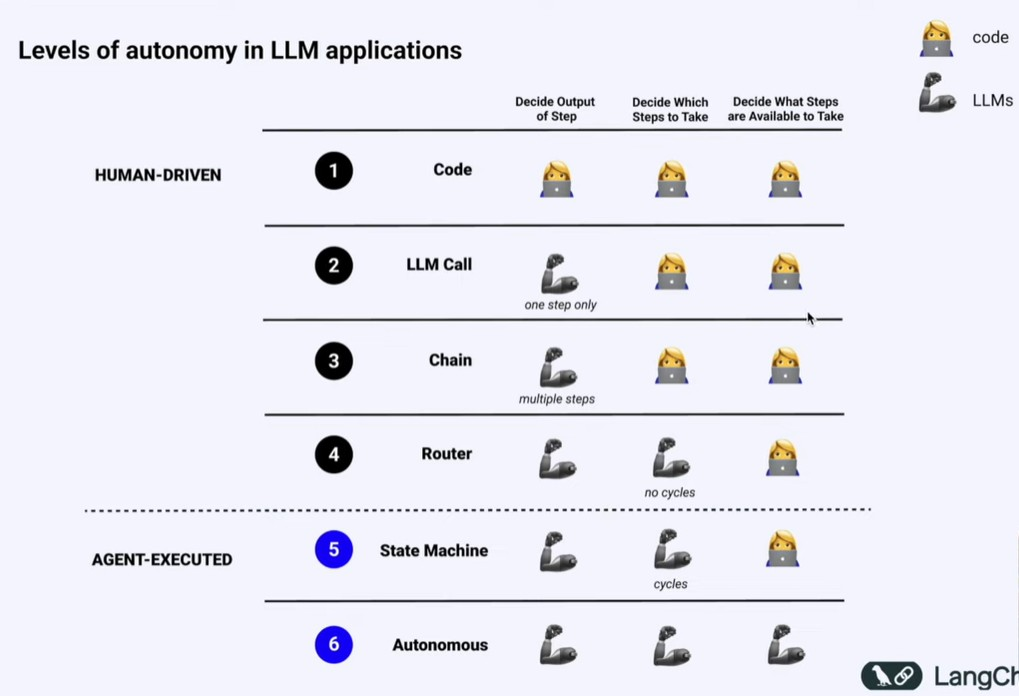
\includegraphics[width=\linewidth,keepaspectratio]{langgraph5}

{\tiny (Ref: LangGraph Crash Course - Harish Neel)}

\end{center}	  


\end{frame}


%%%%%%%%%%%%%%%%%%%%%%%%%%%%%%%%%%%%%%%%%%%%%%%%%%%%%%%%%%%
\begin{frame}[fragile]\frametitle{Introduction to AI Agents}
      \begin{itemize}
        \item AI agents are the problem solvers of the AI world
        \item They are capable of autonomous thinking and decision-making
        \item Unlike chains and routers, agents don't just follow specific instructions
        \item Agents can decide for themselves what steps to take
        \item They represent AI systems that can make independent decisions
        \item Agents take problem-solving capabilities a step further than traditional AI systems
      \end{itemize}
\end{frame}

%%%%%%%%%%%%%%%%%%%%%%%%%%%%%%%%%%%%%%%%%%%%%%%%%%%%%%%%%%%
\begin{frame}[fragile]\frametitle{Understanding Tools for AI Agents}
      \begin{itemize}
        \item Tools are specific functions that agents use to complete tasks
        \item Analogy: Like a chef's kitchen tools - knife for cutting, oven for baking, blender for mixing
        \item Tools provide special abilities to AI agents
        \item Common tools include calculator, search engine, and calendar functions
        \item Tools extend the agent's capabilities beyond basic reasoning
        \item They enable agents to interact with external systems and perform specific operations
      \end{itemize}
\end{frame}

%%%%%%%%%%%%%%%%%%%%%%%%%%%%%%%%%%%%%%%%%%%%%%%%%%%%%%%%%%%
\begin{frame}[fragile]\frametitle{The ReAct Agent Pattern}
      \begin{itemize}
        \item ReAct stands for Reasoning plus Acting
        \item One of the best-known patterns for building AI agents today
        \item Mimics how human beings think and solve problems
        \item Combines reasoning capabilities with action execution
        \item Provides a structured approach to agent decision-making
        \item Forms the foundation for many modern AI agent implementations
      \end{itemize}
\end{frame}

%%%%%%%%%%%%%%%%%%%%%%%%%%%%%%%%%%%%%%%%%%%%%%%%%%%%%%%%%%%
\begin{frame}[fragile]\frametitle{ReAct Pattern Components}
      \begin{itemize}
        \item \textbf{Think}: LLM first thinks about the user's prompt or problem
        \item \textbf{Action}: LLM decides if it can answer directly or needs a tool
        \item \textbf{Action Input}: LLM provides input arguments for the selected tool
        \item \textbf{Observe}: LLM observes the output of the tool execution
        \item Cycle continues until the final answer is reached
        \item Mirrors human problem-solving approach: think → act → observe
      \end{itemize}
\end{frame}

%%%%%%%%%%%%%%%%%%%%%%%%%%%%%%%%%%%%%%%%%%%%%%%%%%%%%%%%%%%
\begin{frame}[fragile]\frametitle{ReAct Pattern Workflow}
      \begin{itemize}
        \item Human problem-solving mimicry: identify problem, determine action, observe results
        \item If answer is found, the cycle ends
        \item If answer is not found, the cycle repeats with new thinking
        \item Control flow: LLM suggests → System executes → Results return to LLM
        \item LLM maintains complete context of all previous think-action-observation cycles
        \item Multi-step problems require multiple cycles until resolution
      \end{itemize}
\end{frame}

%%%%%%%%%%%%%%%%%%%%%%%%%%%%%%%%%%%%%%%%%%%%%%%%%%%%%%%%%%%
\begin{frame}[fragile]\frametitle{Control Flow in ReAct Pattern}
      \begin{itemize}
        \item LLM acts as the reasoning component but doesn't execute tools directly
        \item LangChain system handles the actual tool execution
        \item LLM provides arguments, system executes with those arguments
        \item Tool execution output is returned to the LLM for observation
        \item LLM has full context of all previous interactions
        \item System manages the orchestration between reasoning and action
      \end{itemize}
\end{frame}

%%%%%%%%%%%%%%%%%%%%%%%%%%%%%%%%%%%%%%%%%%%%%%%%%%%%%%%%%%%
\begin{frame}[fragile]\frametitle{Agent Architecture: Brain + Tools}
      \begin{itemize}
        \item LLM provides the reasoning ability (the "brain")
        \item Tools provide execution capabilities (API calls, Google search, Python functions)
        \item Combination of brain + tools = AI Agent
        \item Reasoning ability alone is not sufficient for complex tasks
        \item Tools extend the agent's reach into the real world
        \item This simple formula creates powerful problem-solving systems
      \end{itemize}
\end{frame}

%%%%%%%%%%%%%%%%%%%%%%%%%%%%%%%%%%%%%%%%%%%%%%%%%%%%%%%%%%%
\begin{frame}[fragile]\frametitle{Practical Implementation Approach}
      \begin{itemize}
        \item Start with building a basic ReAct agent using LangChain
        \item Identify drawbacks and limitations of the basic approach
        \item Understand where LangGraph comes into the picture
        \item Learn what specific problems LangGraph solves
        \item Progress from theory to practical coding implementation
        \item Build understanding through hands-on experience
      \end{itemize}
\end{frame}

%%%%%%%%%%%%%%%%%%%%%%%%%%%%%%%%%%%%%%%%%%%%%%%%%%%%%%%%%%%
\begin{frame}[fragile]\frametitle{Practical Implementation: LangChain ReACT way}

\begin{center}
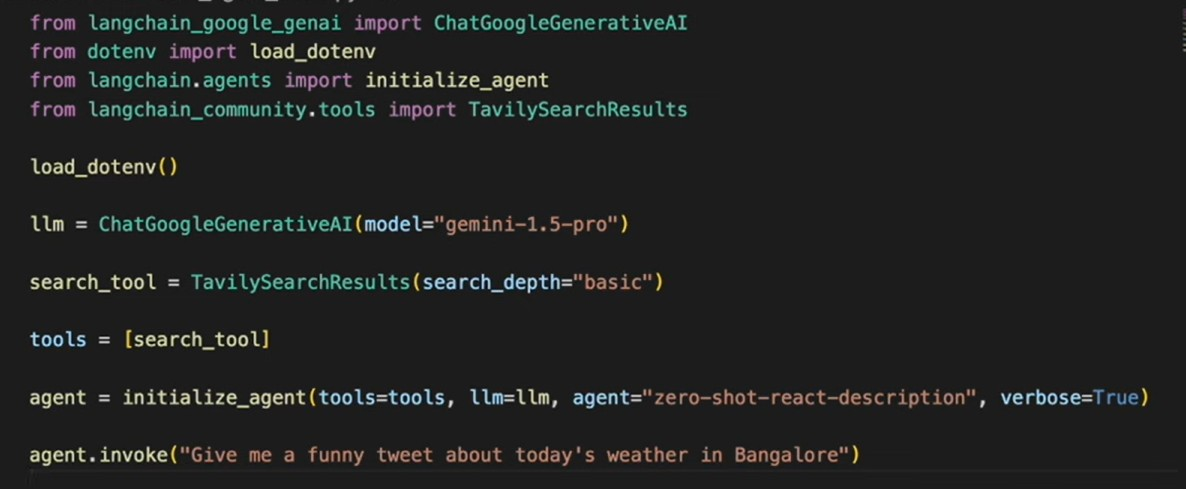
\includegraphics[width=\linewidth,keepaspectratio]{langgraph6}


{\tiny (Ref: LangGraph Crash Course - Harish Neel)}

\end{center}	  

\end{frame}

%%%%%%%%%%%%%%%%%%%%%%%%%%%%%%%%%%%%%%%%%%%%%%%%%%%%%%%%%%%
\begin{frame}[fragile]\frametitle{Practical Implementation: LangChain ReACT way}

ReACT is nothing but a prompting technique.

\begin{center}
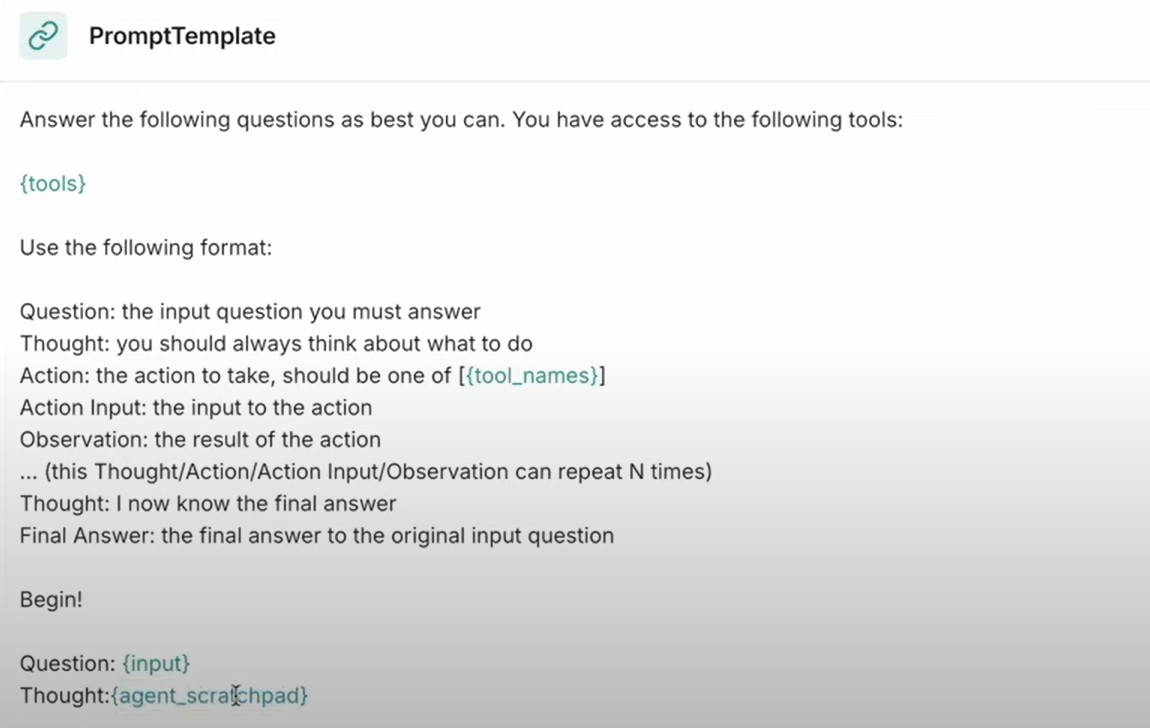
\includegraphics[width=0.8\linewidth,keepaspectratio]{langgraph9}


{\tiny (Ref: LangGraph Crash Course - Harish Neel)}

\end{center}	  

\end{frame}

%%%%%%%%%%%%%%%%%%%%%%%%%%%%%%%%%%%%%%%%%%%%%%%%%%%%%%%%%%%
\begin{frame}[fragile]\frametitle{Study Output}

\begin{center}
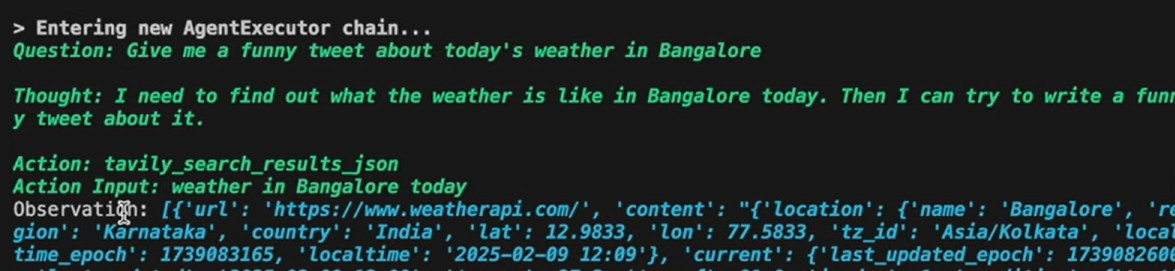
\includegraphics[width=\linewidth,keepaspectratio]{langgraph7}

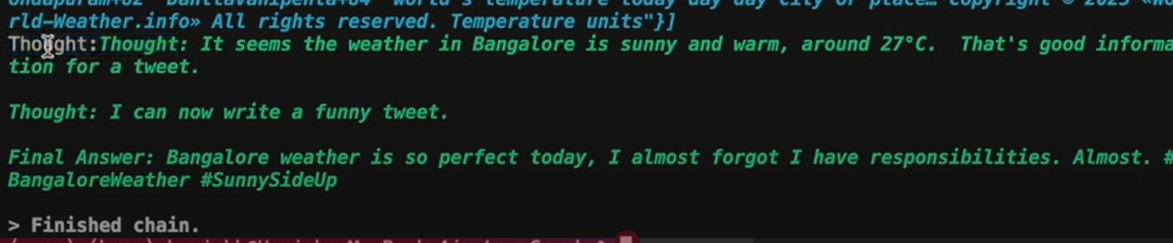
\includegraphics[width=\linewidth,keepaspectratio]{langgraph8}

{\tiny (Ref: LangGraph Crash Course - Harish Neel)}

\end{center}	  

\end{frame}


%%%%%%%%%%%%%%%%%%%%%%%%%%%%%%%%%%%%%%%%%%%%%%%%%%%%%%%%%%%
\begin{frame}[fragile]\frametitle{Key Takeaways}
      \begin{itemize}
        \item Agents represent autonomous AI that can make independent decisions
        \item ReAct pattern provides a structured framework for agent behavior
        \item Tools are essential for extending agent capabilities beyond reasoning
        \item The think-action-observe cycle mirrors human problem-solving
        \item LangChain orchestrates the interaction between reasoning and execution
        \item Understanding these fundamentals is crucial for advanced agent development
      \end{itemize}
\end{frame}

%%%%%%%%%%%%%%%%%%%%%%%%%%%%%%%%%%%%%%%%%%%%%%%%%%%%%%%%%%%
\begin{frame}[fragile]\frametitle{React Agents: Advantages and Flexibility}
      \begin{itemize}
        \item React agents offer high flexibility - any state execution is possible
        \item Dynamic tool execution order: tool 1 → tool 2 or tool 2 → tool 1
        \item Example: SpaceX launch query could execute Tavily Search first, then get current time
        \item Alternative execution: get current system time first, then perform research
        \item Agents can adapt execution flow based on problem requirements
        \item Multiple valid execution paths for the same problem
        \item State transitions are not predetermined or fixed
      \end{itemize}
\end{frame}

%%%%%%%%%%%%%%%%%%%%%%%%%%%%%%%%%%%%%%%%%%%%%%%%%%%%%%%%%%%
\begin{frame}[fragile]\frametitle{React Agents: Drawbacks and Reliability Issues}
      \begin{itemize}
        \item High flexibility often leads to reduced reliability
        \item Infinite loops are a significant problem with React agents
        \item Tools can get called repeatedly without proper termination
        \item Common causes of infinite loops:
        \begin{itemize}
            \item Incorrectly defined tools
            \item Insufficient LLM capabilities
            \item Poor prompting without clear end conditions
        \end{itemize}
        \item Execution is not completely under developer control
        \item Google Gemini example showed tool being called infinitely until stopped
      \end{itemize}
\end{frame}

%%%%%%%%%%%%%%%%%%%%%%%%%%%%%%%%%%%%%%%%%%%%%%%%%%%%%%%%%%%
\begin{frame}[fragile]\frametitle{Chains vs React Agents: The Trade-off}
      \begin{itemize}
        \item \textbf{Chains}: Fixed assembly line approach
        \begin{itemize}
            \item Low flexibility but high reliability
            \item Predetermined execution sequence
            \item Predictable outcomes
        \end{itemize}
        \item \textbf{React Agents}: Dynamic execution approach
        \begin{itemize}
            \item High flexibility but low reliability
            \item Unpredictable execution paths
            \item Potential for infinite loops
        \end{itemize}
        \item Need for a solution combining best of both worlds
        \item Requirement: flexible yet reliable system
      \end{itemize}
\end{frame}

%%%%%%%%%%%%%%%%%%%%%%%%%%%%%%%%%%%%%%%%%%%%%%%%%%%%%%%%%%%
\begin{frame}[fragile]\frametitle{Introducing LangGraph: Best of Both Worlds}
      \begin{itemize}
        \item LangGraph provides flexibility with reliability
        \item Uses state machine architecture for controlled execution
        \item Bridges the gap between rigid chains and unpredictable React agents
        \item Maintains dynamic execution while ensuring controllability
        \item Framework designed for building controllable agent workflows
        \item Combines the advantages while minimizing the drawbacks
        \item Graph-based approach enables structured flexibility
      \end{itemize}
\end{frame}

%%%%%%%%%%%%%%%%%%%%%%%%%%%%%%%%%%%%%%%%%%%%%%%%%%%%%%%%%%%
\begin{frame}[fragile]\frametitle{LangGraph: Definition and Core Purpose}
      \begin{itemize}
        \item \textbf{Definition}: Framework for building controllable, persistent agent workflows
        \item Built-in support for human interaction and streaming
        \item Comprehensive state management capabilities
        \item Uses graph data structure as foundation
        \item Basic structure: Start Node → Agent → Action → Continue/End
        \item Enables creation of sophisticated agent workflows
        \item Designed for production-ready AI applications
      \end{itemize}
\end{frame}

%%%%%%%%%%%%%%%%%%%%%%%%%%%%%%%%%%%%%%%%%%%%%%%%%%%%%%%%%%%
\begin{frame}[fragile]\frametitle{LangGraph Key Features: Looping and Branching}
      \begin{itemize}
        \item \textbf{Looping and Branching Abilities}:
        \begin{itemize}
            \item Supports conditional statements and loop structures
            \item Dynamic execution paths based on current state
            \item Enables complex decision-making workflows
        \end{itemize}
        \item \textbf{State Persistence}:
        \begin{itemize}
            \item Automatic state saving and management
            \item Support for pause and resume functionality
            \item Ideal for long-running conversations and processes
        \end{itemize}
        \item Provides controlled flexibility unlike pure React agents
      \end{itemize}
\end{frame}

%%%%%%%%%%%%%%%%%%%%%%%%%%%%%%%%%%%%%%%%%%%%%%%%%%%%%%%%%%%
\begin{frame}[fragile]\frametitle{LangGraph Key Features: Interaction and Integration}
      \begin{itemize}
        \item \textbf{Human-Machine Interaction Support}:
        \begin{itemize}
            \item Insert human review during execution
            \item State editing and modification capabilities
            \item Flexible interaction control mechanisms
        \end{itemize}
        \item \textbf{Streaming Processing}:
        \begin{itemize}
            \item Real-time feedback on execution status
            \item Enhanced user experience through streaming output
        \end{itemize}
        \item \textbf{Seamless LangChain Integration}:
        \begin{itemize}
            \item Reuses existing LangChain components
            \item Supports LangChain Expression Language
            \item Rich tool and model support
        \end{itemize}
      \end{itemize}
\end{frame}

%%%%%%%%%%%%%%%%%%%%%%%%%%%%%%%%%%%%%%%%%%%%%%%%%%%%%%%%%%%
\begin{frame}[fragile]\frametitle{Why Graph Data Structure?}
      \begin{itemize}
        \item Graph structure chosen based on research paper evidence
        \item Most complex problem-solving research uses graph data structures
        \item Provides flexibility while maintaining controllability
        \item Enables autonomous decision-making capabilities
        \item Natural fit for agent workflow representation
        \item Balances flexibility with structured control
        \item Supports complex branching and conditional logic
        \item Research-proven approach for difficult AI problems
      \end{itemize}
\end{frame}

%%%%%%%%%%%%%%%%%%%%%%%%%%%%%%%%%%%%%%%%%%%%%%%%%%%%%%%%%%%
\begin{frame}[fragile]\frametitle{LangGraph Core Components Overview}
      \begin{itemize}
        \item \textbf{Four Core Components}:
        \begin{itemize}
            \item Nodes
            \item Edges  
            \item Conditional Edges
            \item State
        \end{itemize}
        \item Components work together to create controllable workflows
        \item Each component serves a specific purpose in graph execution
        \item Understanding these components is crucial for LangGraph mastery
        \item Will be demonstrated through Reflection Agent Pattern example
      \end{itemize}
\end{frame}

%%%%%%%%%%%%%%%%%%%%%%%%%%%%%%%%%%%%%%%%%%%%%%%%%%%%%%%%%%%
\begin{frame}[fragile]\frametitle{Reflection Agent Pattern: Example Overview}
      \begin{itemize}
        \item \textbf{Pattern Components}:
        \begin{itemize}
            \item Generation Component: Creates content (e.g., tweets)
            \item Criticism Component: Evaluates and suggests improvements
        \end{itemize}
        \item \textbf{Workflow}:
        \begin{itemize}
            \item Agent generates initial tweet
            \item Critic evaluates quality and provides feedback
            \item Generator improves tweet based on criticism
            \item Process loops until quality threshold is met
        \end{itemize}
        \item Example of iterative improvement through agent collaboration
        \item Demonstrates practical application of LangGraph components
      \end{itemize}
\end{frame}

%%%%%%%%%%%%%%%%%%%%%%%%%%%%%%%%%%%%%%%%%%%%%%%%%%%%%%%%%%%
\begin{frame}[fragile]\frametitle{Core Components: Nodes}
      \begin{itemize}
        \item \textbf{Nodes}: Fundamental execution units in the graph
        \item Examples in Reflection Agent Pattern:
        \begin{itemize}
            \item Start Node: Entry point of the workflow
            \item Generate Tweet LLM: Content creation node
            \item Criticize Tweet LLM: Evaluation node
            \item End Node: Termination point
        \end{itemize}
        \item Each node represents a specific operation or LLM call
        \item Nodes contain the actual logic and processing
        \item Can be simple operations or complex LLM interactions
      \end{itemize}
\end{frame}

%%%%%%%%%%%%%%%%%%%%%%%%%%%%%%%%%%%%%%%%%%%%%%%%%%%%%%%%%%%
\begin{frame}[fragile]\frametitle{Core Components: Edges}
      \begin{itemize}
        \item \textbf{Edges}: Connections between nodes in the graph
        \item Represent the flow of execution from one node to another
        \item Shown as lines connecting different nodes
        \item Define the possible paths through the workflow
        \item Ensure proper sequence of operations
        \item Can be simple directional connections
        \item Enable linear workflow progression
        \item Essential for maintaining execution order
      \end{itemize}
\end{frame}

%%%%%%%%%%%%%%%%%%%%%%%%%%%%%%%%%%%%%%%%%%%%%%%%%%%%%%%%%%%
\begin{frame}[fragile]\frametitle{Core Components: Conditional Edges}
      \begin{itemize}
        \item \textbf{Conditional Edges}: Decision points in the workflow
        \item Enable branching based on specific conditions
        \item In Reflection Agent example:
        \begin{itemize}
            \item After tweet generation, can go to criticism OR end
            \item Decision based on iteration count or quality threshold
        \end{itemize}
        \item Represented by dotted lines in diagrams
        \item Allow for dynamic execution paths
        \item Essential for implementing complex decision logic
        \item Enable loops and conditional branching
      \end{itemize}
\end{frame}

%%%%%%%%%%%%%%%%%%%%%%%%%%%%%%%%%%%%%%%%%%%%%%%%%%%%%%%%%%%
\begin{frame}[fragile]\frametitle{Core Components: State Management}
      \begin{itemize}
        \item \textbf{State}: Maintains context throughout workflow execution
        \item Preserves information between node executions
        \item In Reflection Agent Pattern:
        \begin{itemize}
            \item Stores generated tweet content
            \item Maintains criticism feedback
            \item Tracks iteration count
            \item Preserves conversation context
        \end{itemize}
        \item Enables nodes to access and modify shared information
        \item Critical for maintaining workflow coherence
        \item Supports complex, stateful operations
      \end{itemize}
\end{frame}

%%%%%%%%%%%%%%%%%%%%%%%%%%%%%%%%%%%%%%%%%%%%%%%%%%%%%%%%%%%
\begin{frame}[fragile]\frametitle{Summary and Next Steps}
      \begin{itemize}
        \item \textbf{Key Learnings}:
        \begin{itemize}
            \item React agents: flexible but unreliable
            \item LangGraph: combines flexibility with reliability
            \item Graph structure enables controlled autonomous decision-making
            \item Four core components: Nodes, Edges, Conditional Edges, State
        \end{itemize}
        \item \textbf{Upcoming Topics}:
        \begin{itemize}
            \item Deep dive into Reflection Agent Pattern
            \item Hands-on implementation and coding
            \item Real-world applications and use cases
        \end{itemize}
      \end{itemize}
\end{frame}

%%%%%%%%%%%%%%%%%%%%%%%%%%%%%%%%%%%%%%%%%%%%%%%%%%%%%%%%%%%
\begin{frame}[fragile]\frametitle{Graph Data Structures}
      \begin{itemize}
        \item Understanding graph-based architectures
        \item Directed Acyclic Graphs (DAGs) vs Cyclical Graphs
        \item Graph theory applications in AI agents
        \item Data flow management in graph structures
        \item Node relationships and connections
        \item State management across graph nodes
        \item Prerequisites for LangGraph implementation
      \end{itemize}
\end{frame}

%%%%%%%%%%%%%%%%%%%%%%%%%%%%%%%%%%%%%%%%%%%%%%%%%%%%%%%%%%%
\begin{frame}[fragile]\frametitle{What is LangGraph and Why Use It?}
      \begin{itemize}
        \item LangGraph: Advanced framework for building AI agent workflows
        \item Limitations of traditional LangChain approaches
        \item Enhanced flexibility and control over agent behavior
        \item Support for complex multi-step reasoning processes
        \item Better state management and workflow orchestration
        \item Low-level control for custom implementations
        \item Production-ready agent development capabilities
      \end{itemize}
\end{frame}

%%%%%%%%%%%%%%%%%%%%%%%%%%%%%%%%%%%%%%%%%%%%%%%%%%%%%%%%%%%%%%%%%%%%%%%%%%%%%%%%%%
\begin{frame}\frametitle{What is LangGraph?}

\begin{itemize}
\item Building state-ful multi agent applications using LLMs (Large Language Models)
\item So, components are not in `chain' as in LangChain (ie Sequential) but can a Graph.
\item Like Workflow modeling or orchestration
\end{itemize}

\begin{center}
\includegraphics[width=0.8\linewidth,keepaspectratio]{langgraph1}
\end{center}	  


{\tiny (Ref: Introduction to LangGraph | Building an AI Generated Podcast - Prompt Circle AI)}
\end{frame}

%%%%%%%%%%%%%%%%%%%%%%%%%%%%%%%%%%%%%%%%%%%%%%%%%%%%%%%%%%%
\begin{frame}[fragile]\frametitle{Introduction to LangGraph}
      \begin{itemize}
        \item LangGraph is a graph-based framework for building complex LLM applications
        \item Represents AI workflows as directed graphs with nodes, edges, and data states
        \item Addresses limitations of LCEL and AgentExecutor in complex scenarios
        \item Provides intuitive and flexible approach to constructing conversational flows
        \item Supports looping, branching, and dynamic execution paths
        \item Enables state persistence and human-machine interaction
        \item Seamlessly integrates with existing LangChain ecosystem
        \item Offers streaming processing and real-time feedback capabilities
      \end{itemize}
\end{frame}

%%%%%%%%%%%%%%%%%%%%%%%%%%%%%%%%%%%%%%%%%%%%%%%%%%%%%%%%%%%
\begin{frame}[fragile]\frametitle{Limitations of LCEL Chain Expressions}
      \begin{itemize}
        \item Linear processes with predefined execution order
        \item Difficulty in dynamic routing and conditional branching
        \item Complex state management in multi-turn conversations
        \item Manual state passing and updates increase code complexity
        \item Non-intuitive tool integration and coordination
        \item Nested tools create highly complex LCEL expressions
        \item Limited flexibility for dynamic conversational scenarios
        \item Error-prone state management across chain calls
      \end{itemize}
\end{frame}

%%%%%%%%%%%%%%%%%%%%%%%%%%%%%%%%%%%%%%%%%%%%%%%%%%%%%%%%%%%
\begin{frame}[fragile]\frametitle{LCEL Complexity Example}

For example, when constructing a parallel sub-problem optimization chain for a problem decomposition strategy, the complexity of LCEL expressions becomes apparent. This example shows that when the nesting level of tools is slightly deeper, constructing LCEL chains becomes quite complex.

\begin{lstlisting}[language=Python, basicstyle=\tiny]
# Decomposition chain
decomposition_chain = (
    {"question": RunnablePassthrough()}
    | decomposition_prompt
    | ChatOpenAI(model="gpt-4o-mini", temperature=0)
    | StrOutputParser()
    | (lambda x: x.strip().split("\n"))
)
# Sub-question answer generation chain
sub_question_chain = (
    {"context": retriever, "question": RunnablePassthrough()}
    | sub_question_prompt
    | ChatOpenAI(model="gpt-4o-mini")
    | StrOutputParser()
)
# Assembly chain
chain = (
    {"question": RunnablePassthrough(), "context": decomposition_chain}
    | {"questions": RunnablePassthrough(), "answers": sub_question_chain.map()}
    | RunnableLambda(format_qa_pairs)
    | prompt
    | llm_output_str
)
      \end{lstlisting}
\end{frame}

%%%%%%%%%%%%%%%%%%%%%%%%%%%%%%%%%%%%%%%%%%%%%%%%%%%%%%%%%%%
\begin{frame}[fragile]\frametitle{Limitations of AgentExecutor}
      \begin{itemize}
        \item Complex configuration for conversational flows and multi-turn dialogues
        \item Limited dynamic routing capability for conditional branches
        \item Lack of built-in state persistence mechanism
        \item Over-encapsulation with fixed input requirements
        \item Black-box uncontrollability in tool usage order
        \item Cannot insert human interaction during execution
        \item Difficult secondary development due to rigid structure
        \item Must restart from scratch when conversation resumes
      \end{itemize}
\end{frame}


%%%%%%%%%%%%%%%%%%%%%%%%%%%%%%%%%%%%%%%%%%%%%%%%%%%%%%%%%%%%%%%%%%%%%%%%%%%%%%%%%%
\begin{frame}[fragile]\frametitle{Why LangGraph?}

\begin{itemize}
\item Limitations of LCEL and AgentExecutor, need a more flexible and powerful framework to build complex agent applications.
\item Most of the Multi-agent frameworks are rigid, monolithic
\item LangGraph decouples the agents from their orchestration.
\item Here, agents can have different LLMs, can combine even non-LLM services together, can combine agents from other systems such as Autogen or Crew AI etc.
\end{itemize}


{\tiny (Ref: Langgraph: The Agent Orchestrator - Rajib Deb)}

% \begin{lstlisting}
% agent_1 = MyAgent("agent_1")
% agent_2 = MyAgent("agent_2")
% group_chat = [agent_1,agent_2]
% group_chat.invoke("What is GST?")
% \end{lstlisting}

\end{frame}


%%%%%%%%%%%%%%%%%%%%%%%%%%%%%%%%%%%%%%%%%%%%%%%%%%%%%%%%%%%
\begin{frame}[fragile]\frametitle{LangChain vs LangGraph}
\begin{columns}
    \begin{column}[T]{0.6\linewidth}
        \begin{center}
        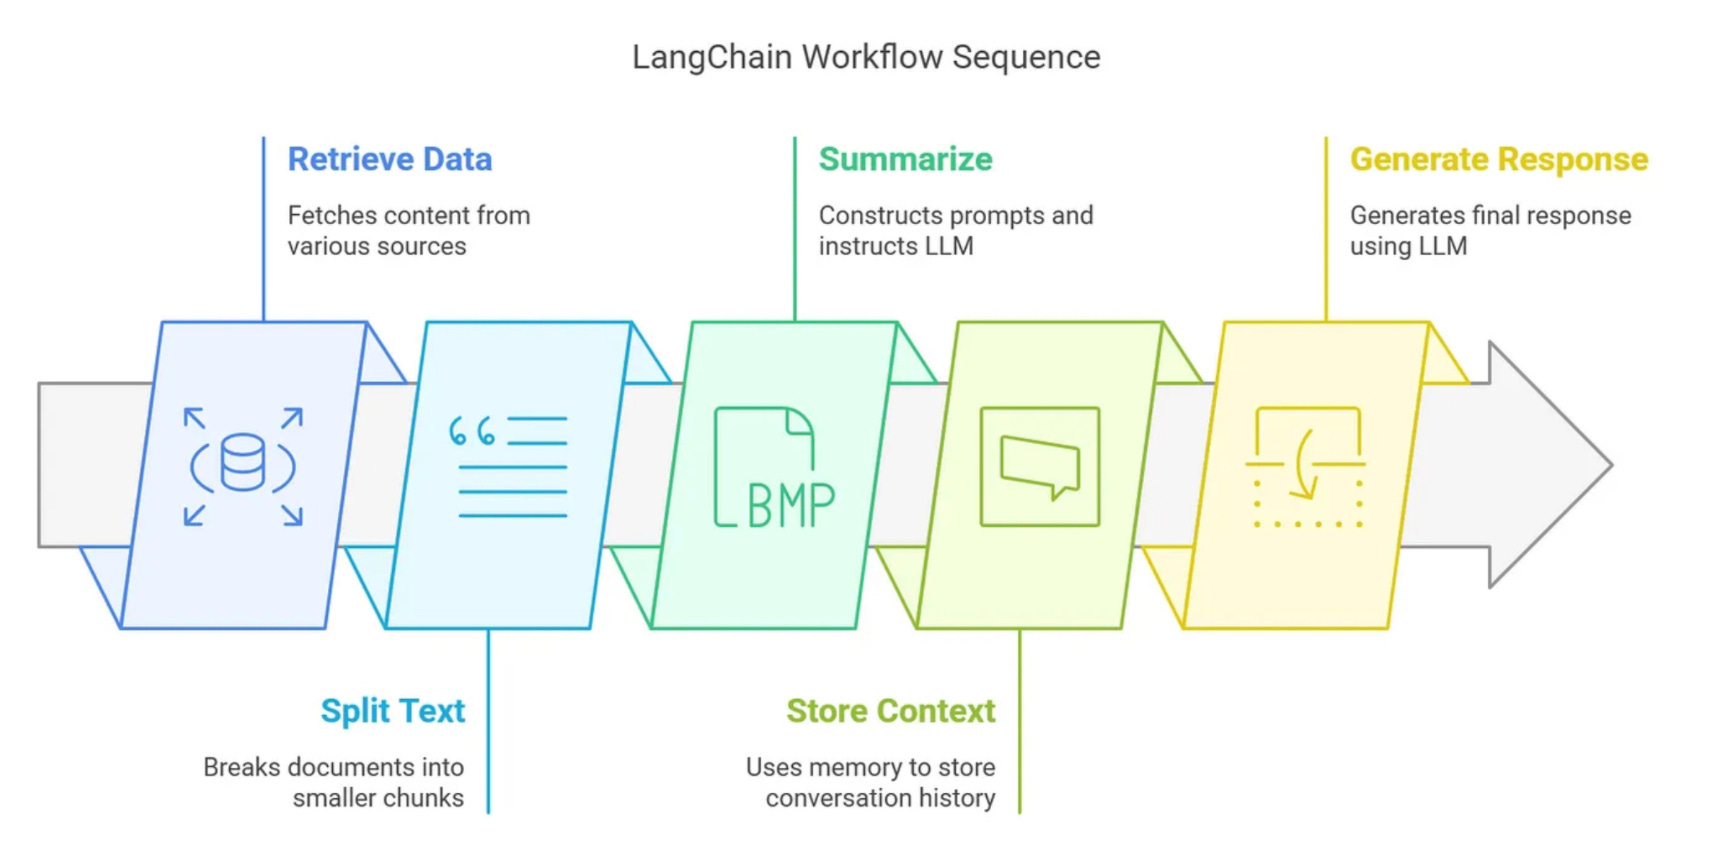
\includegraphics[width=0.8\linewidth,keepaspectratio]{aiagents64}
		
        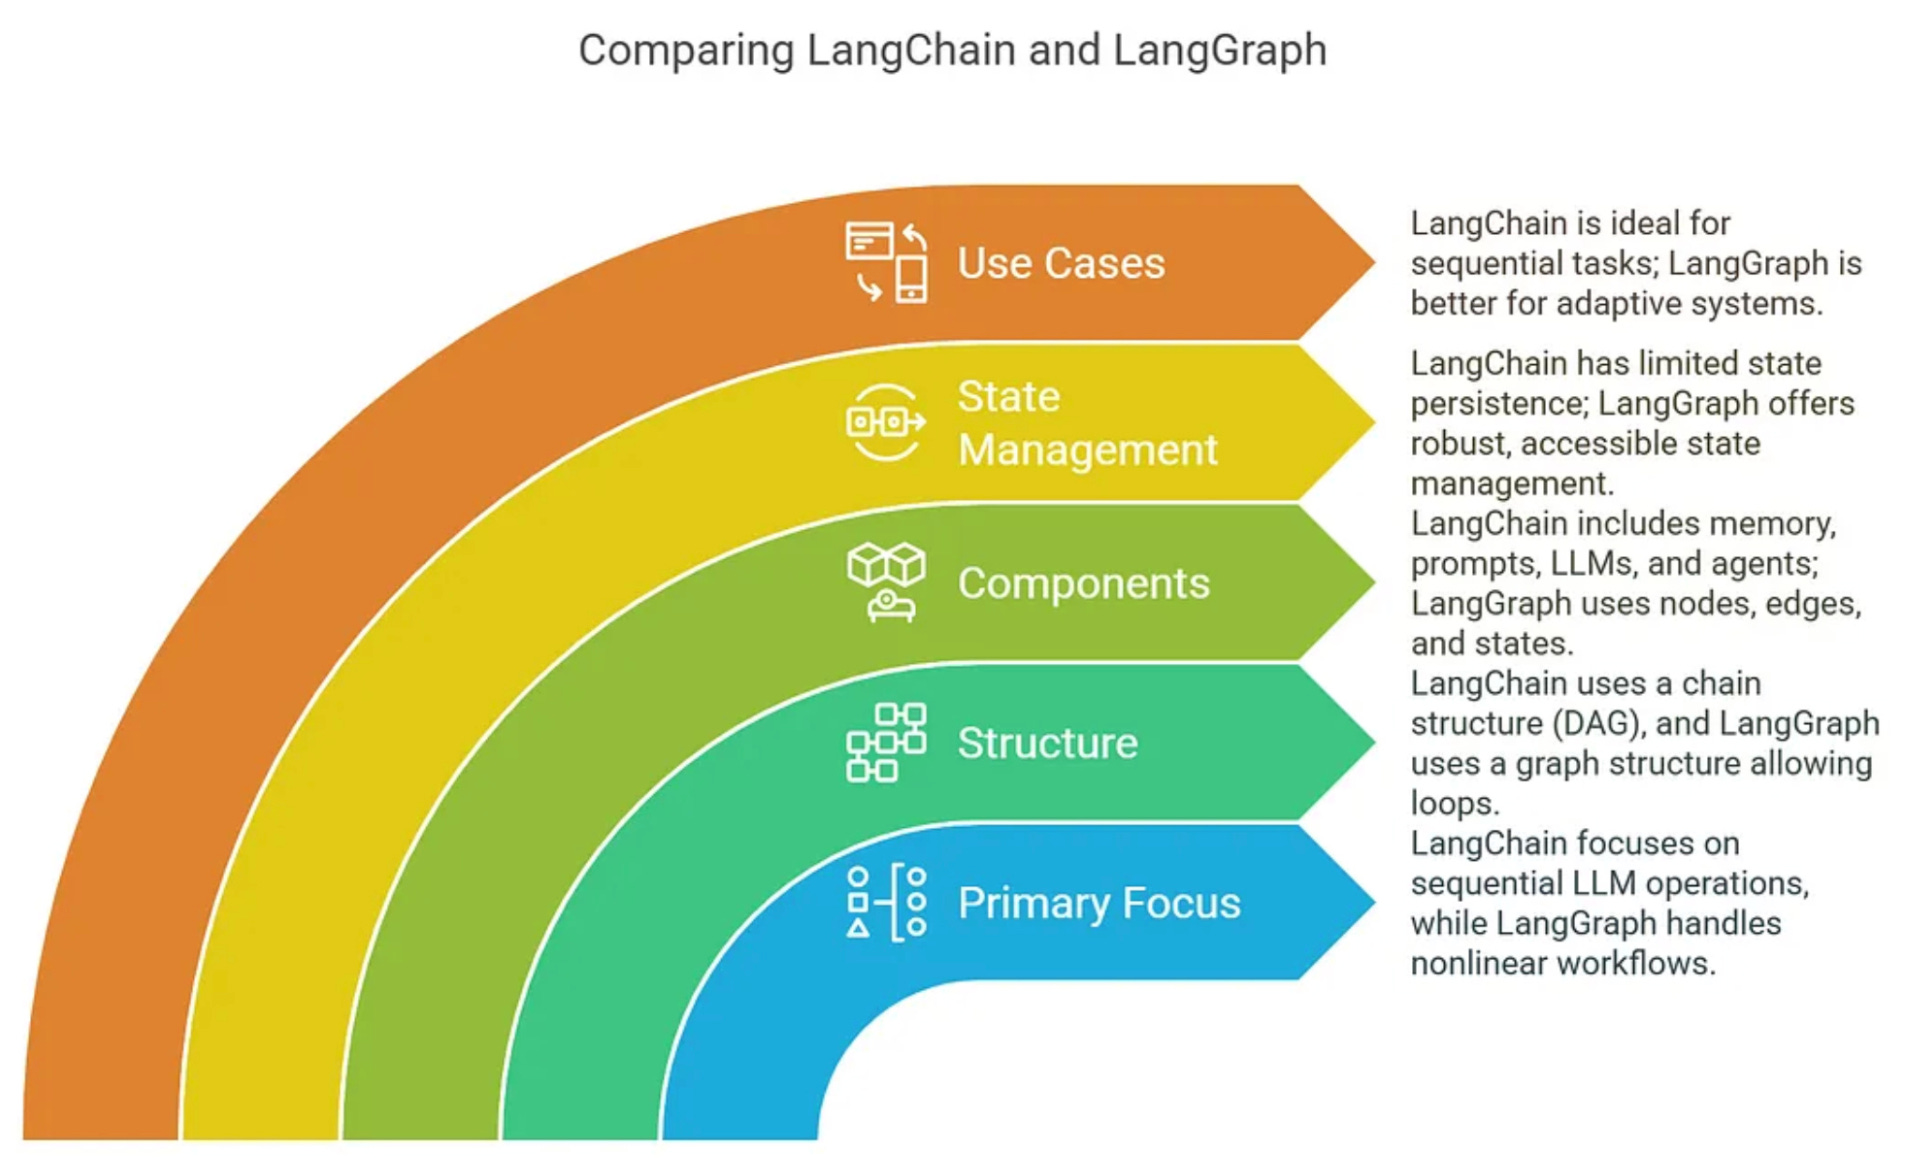
\includegraphics[width=0.8\linewidth,keepaspectratio]{aiagents66}
		
		{\tiny (Ref: Vizuara AI Agents Bootcamp)}
				
        \end{center}    
    \end{column}
    \begin{column}[T]{0.4\linewidth}
        \begin{center}
        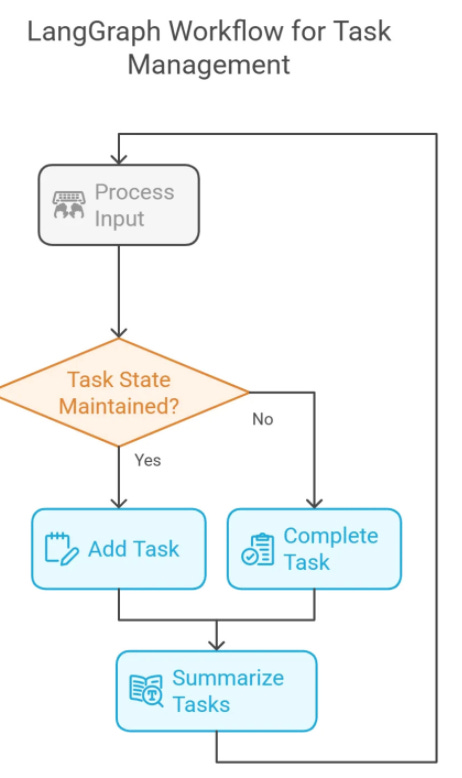
\includegraphics[width=0.8\linewidth,keepaspectratio]{aiagents65}
		
		{\tiny (Ref: Vizuara AI Agents Bootcamp)}
				
        \end{center}    
    \end{column}
  \end{columns}
\end{frame}


%%%%%%%%%%%%%%%%%%%%%%%%%%%%%%%%%%%%%%%%%%%%%%%%%%%%%%%%%%%
\begin{frame}[fragile]\frametitle{LangChain vs LangGraph – Why a New Approach?}

      \begin{itemize}
        \item LangChain excels at straightforward pipelines with fixed sequential tasks (retrieve → summarize → answer)
        \item Real-world workflows aren't always linear - they need branches, loops, and dynamic decision points
        \item LangGraph specializes in stateful, non-linear workflows within the LangChain ecosystem
        \item LangGraph exposes control flow explicitly, allowing fine-grained control over agent behavior
        \item You define a graph of possible steps instead of a rigid chain structure
        \item Agents can revisit nodes or choose different paths dynamically based on conditions
        \item Use LangChain for simple sequences, LangGraph for conditional logic and extended context
        \item LangGraph enables complex multi-agent systems with evolving task flows
      \end{itemize}

\end{frame}

%%%%%%%%%%%%%%%%%%%%%%%%%%%%%%%%%%%%%%%%%%%%%%%%%%%%%%%%%%%
\begin{frame}[fragile]\frametitle{LangGraph Fundamentals: Nodes, Edges \& State}

      \begin{itemize}
        \item \textbf{Nodes (N):} Individual processing steps implemented as Python functions that transform state
        \item Each node encapsulates one sub-task: LLM calls, calculations, file operations, or tool invocations
        \item \textbf{Edges (E):} Directed connections determining execution order and flow between nodes
        \item Edges can be linear progressions or conditional routes based on current state
        \item \textbf{State (S):} Shared data object (dictionary/TypedDict) persisting throughout agent execution
        \item State enables context and memory across workflow, allowing nodes to read previous results
        \item StateGraph ties everything together with designated START and END nodes
        \item This approach handles interactive, conditional loops that static chains struggle with
      \end{itemize}
  

\end{frame}

%%%%%%%%%%%%%%%%%%%%%%%%%%%%%%%%%%%%%%%%%%%%%%%%%%%%%%%%%%%
\begin{frame}[fragile]\frametitle{LangGraph}
\begin{columns}
    \begin{column}[T]{0.5\linewidth}
        \begin{center}
		
        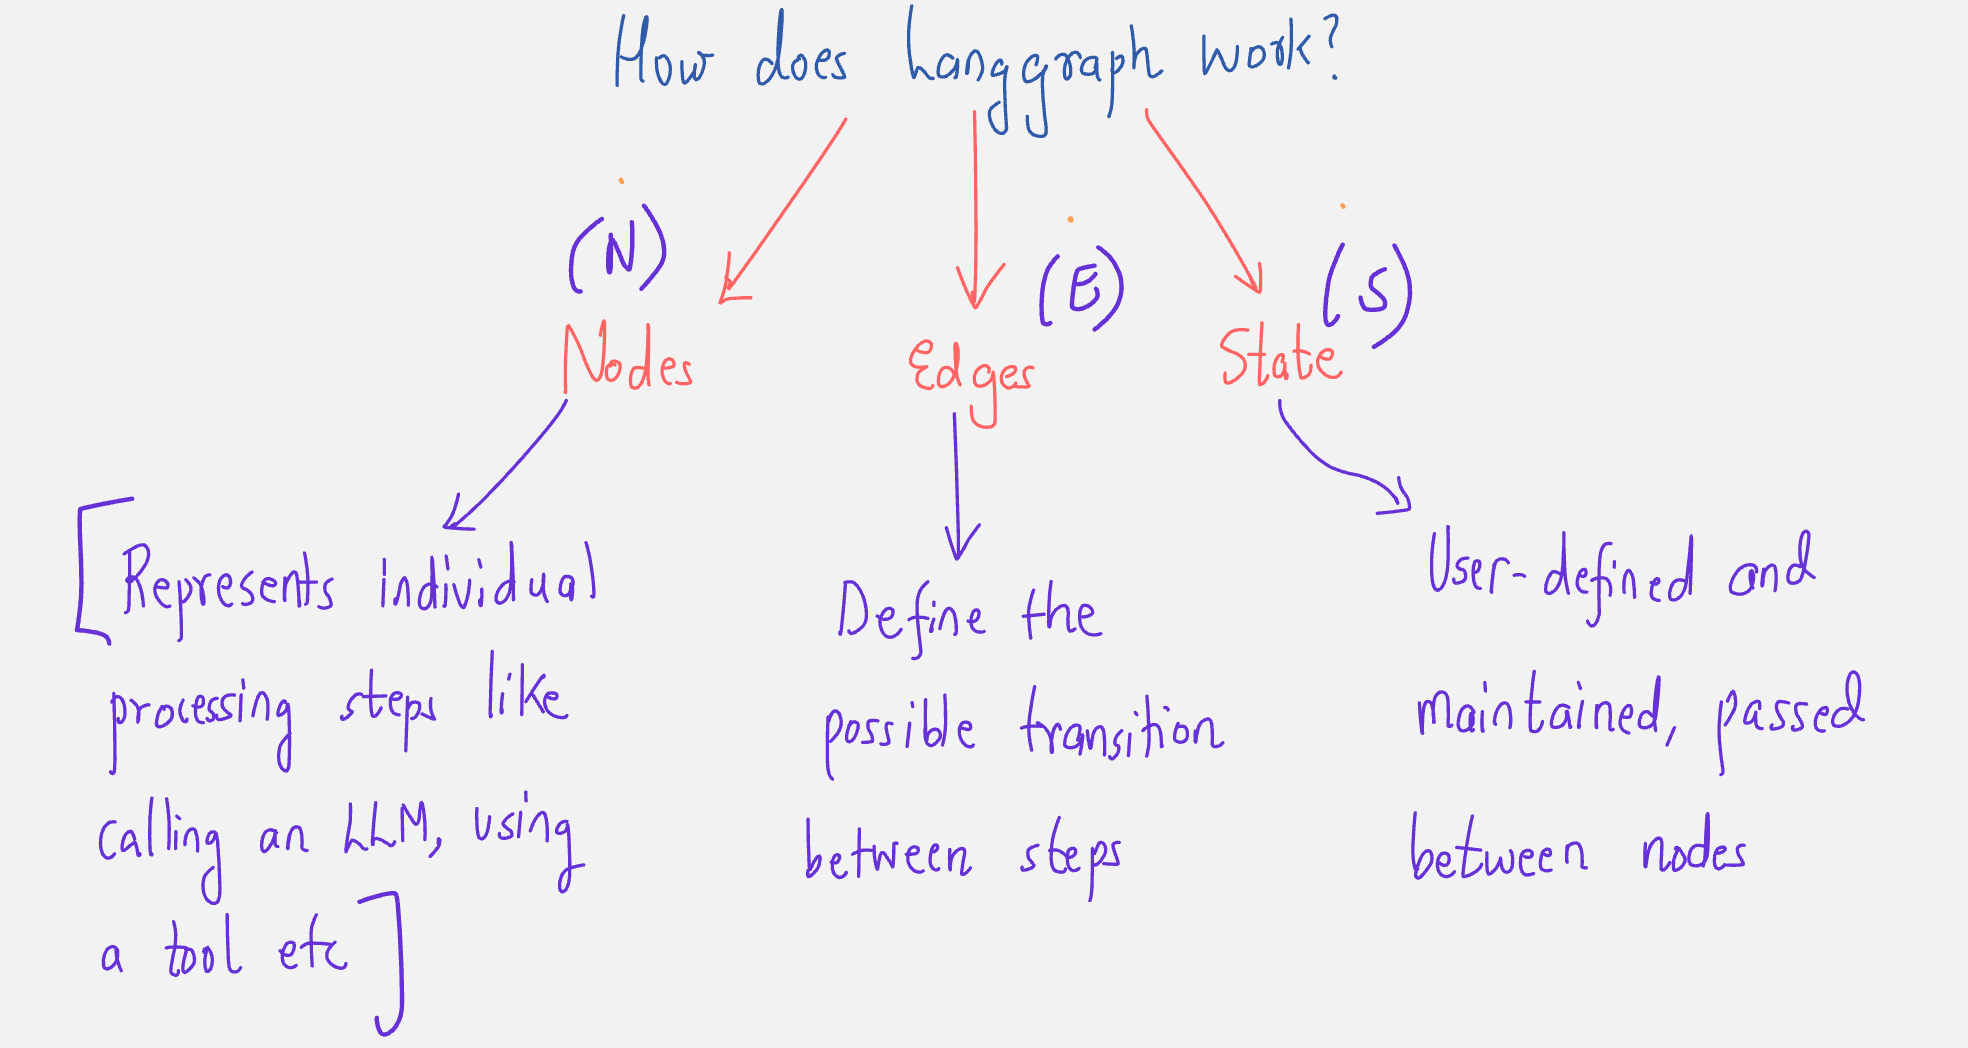
\includegraphics[width=0.8\linewidth,keepaspectratio]{aiagents67}
		
        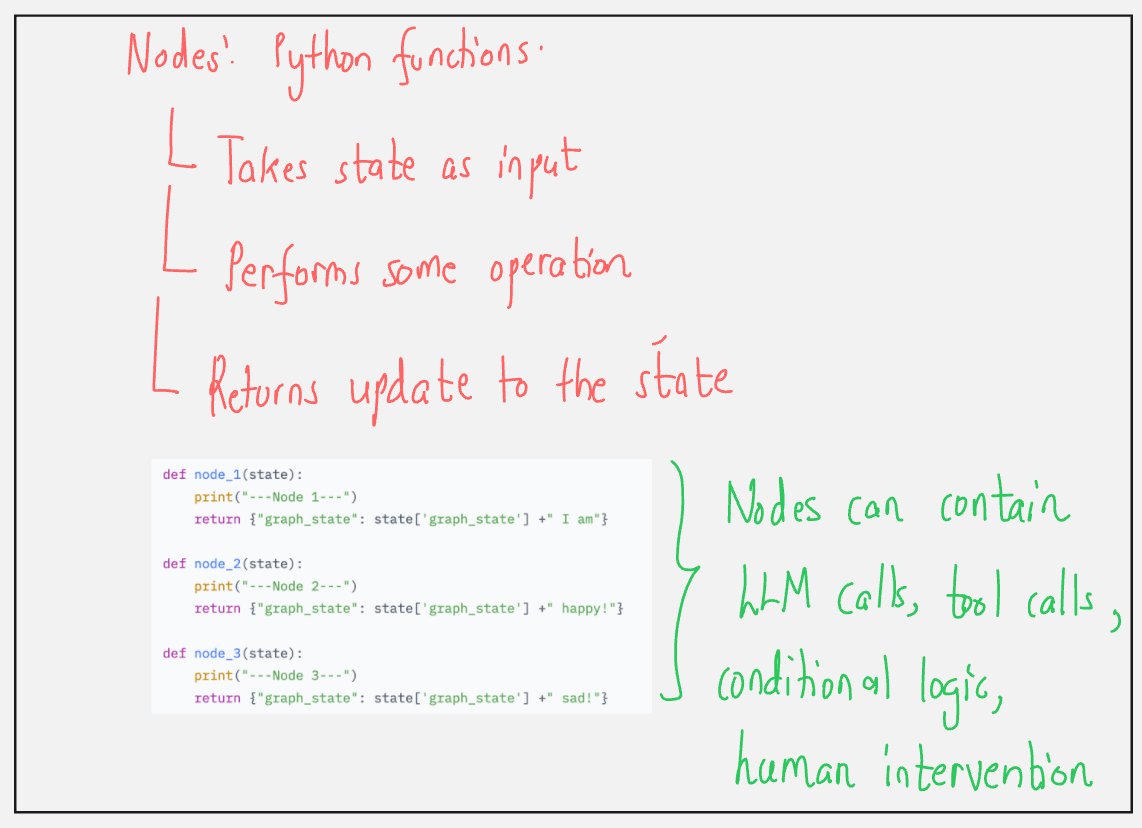
\includegraphics[width=0.8\linewidth,keepaspectratio]{aiagents68}
		
		
		{\tiny (Ref: Vizuara AI Agents Bootcamp)}
				
        \end{center}    
    \end{column}
    \begin{column}[T]{0.5\linewidth}
        \begin{center}
        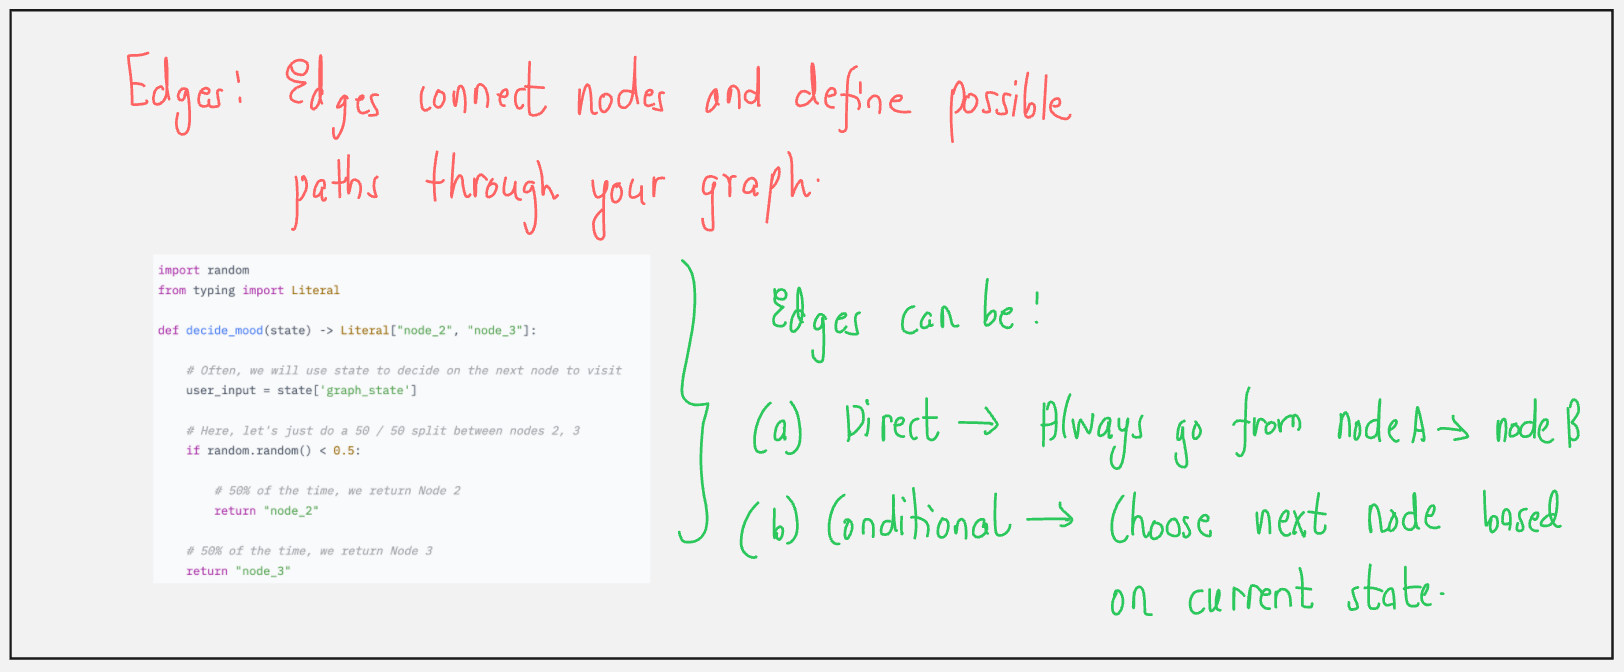
\includegraphics[width=0.8\linewidth,keepaspectratio]{aiagents69}
		
        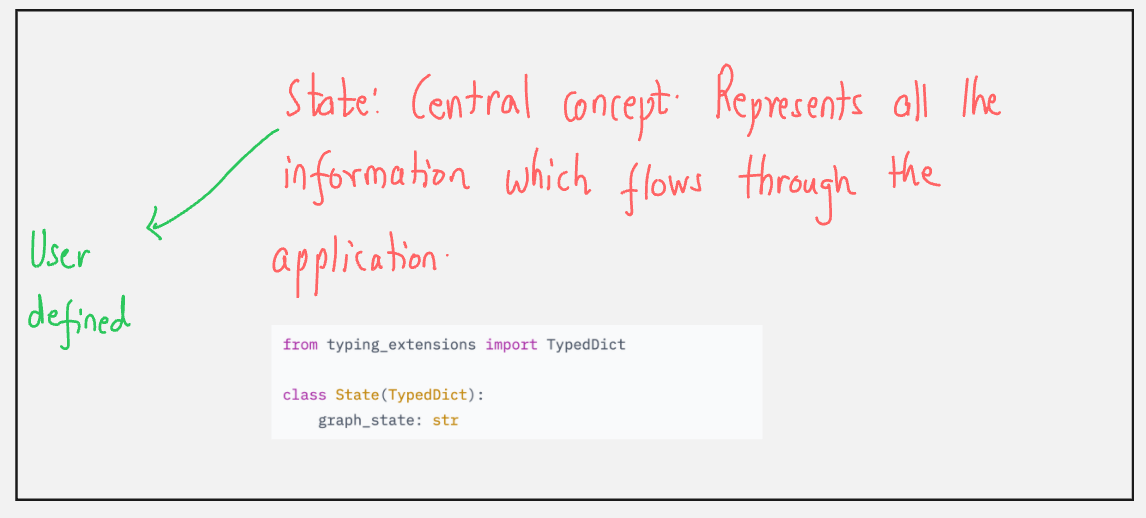
\includegraphics[width=0.8\linewidth,keepaspectratio]{aiagents70}
		
        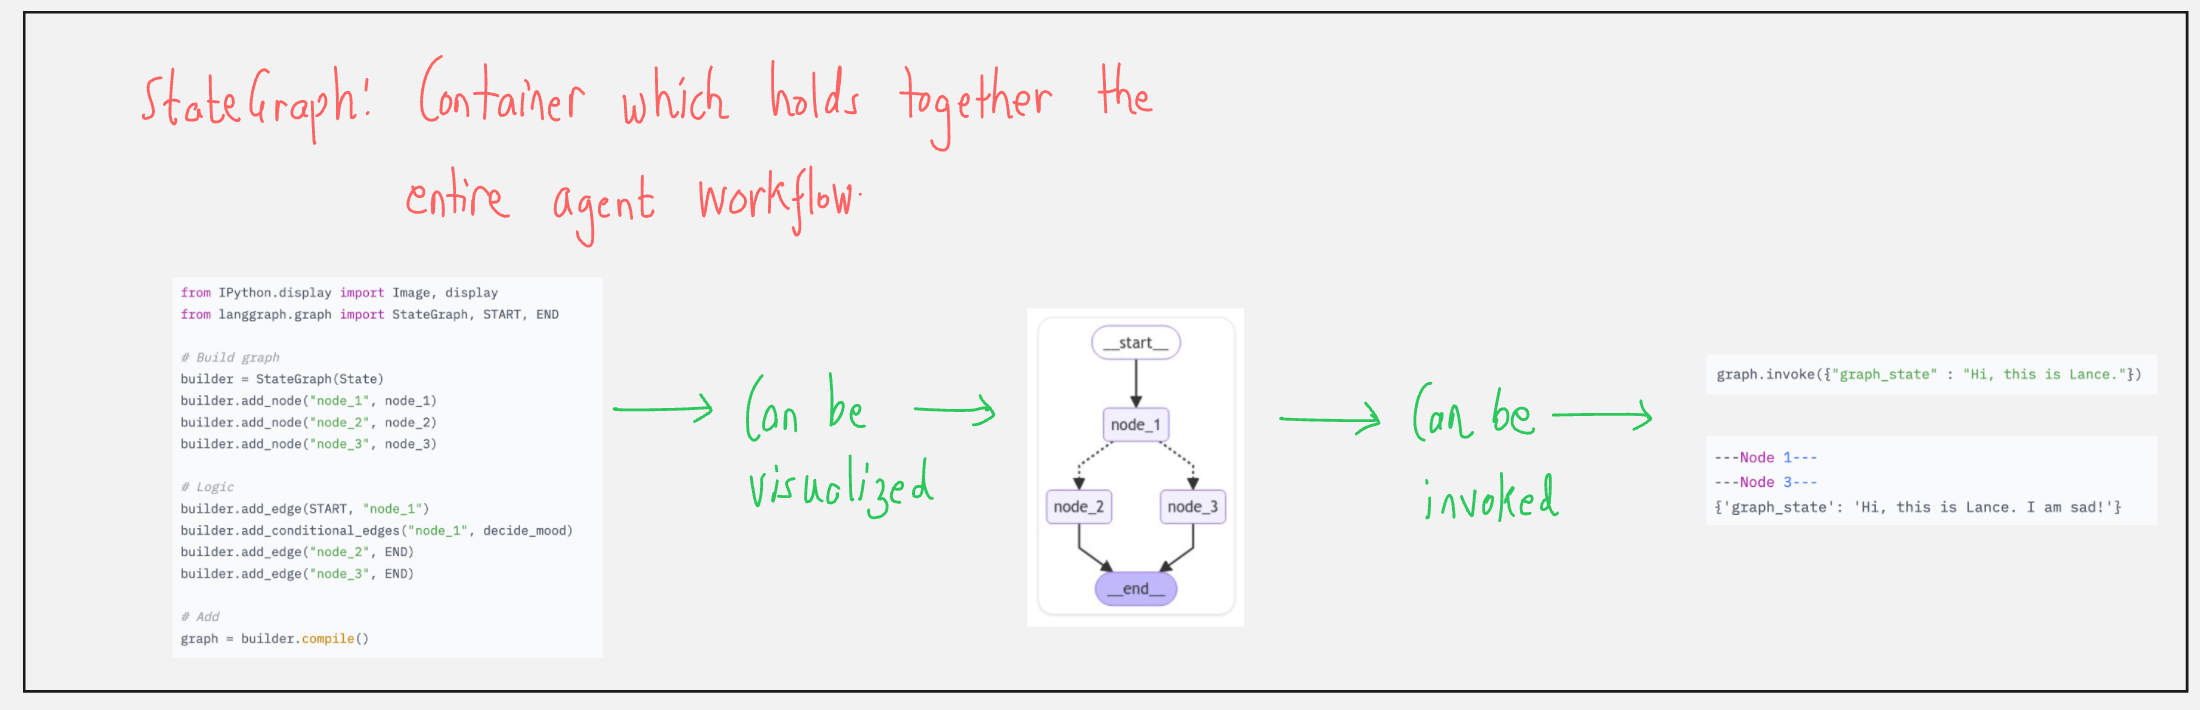
\includegraphics[width=0.8\linewidth,keepaspectratio]{aiagents71}
		
		{\tiny (Ref: Vizuara AI Agents Bootcamp)}
				
        \end{center}    
    \end{column}
  \end{columns}
\end{frame}

%%%%%%%%%%%%%%%%%%%%%%%%%%%%%%%%%%%%%%%%%%%%%%%%%%%%%%%%%%%
\begin{frame}[fragile]\frametitle{Agentic Architecture Patterns}
      \begin{itemize}
        \item Reflection Agent: Self-evaluation and improvement mechanisms
        \item Reflexion Agent: Learning from past experiences
        \item Multi-agent Workflows: Collaborative agent systems
        \item Human-in-the-Loop Patterns: Manual oversight integration
        \item React Patterns: Reasoning and acting frameworks
        \item Chain Exploration: Alternative path discovery
        \item Pattern Selection: Choosing appropriate architectures
      \end{itemize}
\end{frame}

%%%%%%%%%%%%%%%%%%%%%%%%%%%%%%%%%%%%%%%%%%%%%%%%%%%%%%%%%%%
\begin{frame}[fragile]\frametitle{Key LangGraph Terminologies}
      \begin{itemize}
        \item Graph: Overall workflow structure and organization
        \item State: Data persistence and management across nodes
        \item Node: Individual processing units within the graph
        \item Visualization: Graphical representation of workflows
        \item Breakpoints: Debugging and control mechanisms
        \item Edges: Connections and transitions between nodes
        \item Flow Control: Managing execution paths and decisions
      \end{itemize}
\end{frame}

%%%%%%%%%%%%%%%%%%%%%%%%%%%%%%%%%%%%%%%%%%%%%%%%%%%%%%%%%%%
\begin{frame}[fragile]\frametitle{Building LangGraph Chatbot}
      \begin{itemize}
        \item Web search capabilities for real-time information
        \item Complex query routing to human reviewers
        \item Backward chaining for alternative exploration
        \item Human-in-the-loop integration patterns
        \item React pattern implementation for reasoning
        \item Multi-path exploration and decision making
        \item Production-ready chatbot architecture
      \end{itemize}
\end{frame}

%%%%%%%%%%%%%%%%%%%%%%%%%%%%%%%%%%%%%%%%%%%%%%%%%%%%%%%%%%%
\begin{frame}[fragile]\frametitle{Multi-Agent Systems}
      \begin{itemize}
        \item Multiple agent creation and management
        \item Inter-agent communication protocols
        \item Task distribution and coordination
        \item More powerful than CrewAI with greater flexibility
        \item Low-level control for custom workflows
        \item Collaborative problem-solving approaches
        \item Scalable multi-agent architectures
      \end{itemize}
\end{frame}

%%%%%%%%%%%%%%%%%%%%%%%%%%%%%%%%%%%%%%%%%%%%%%%%%%%%%%%%%%%
\begin{frame}[fragile]\frametitle{RAG Integration with LangGraph}
      \begin{itemize}
        \item Corrective RAG (C-RAG): Error correction mechanisms
        \item Adaptive RAG (A-RAG): Dynamic retrieval strategies
        \item Self-RAG: Self-evaluation and improvement
        \item Advanced retrieval and generation patterns
        \item Context-aware information processing
        \item Quality control in RAG implementations
        \item Performance optimization techniques
      \end{itemize}
\end{frame}

%%%%%%%%%%%%%%%%%%%%%%%%%%%%%%%%%%%%%%%%%%%%%%%%%%%%%%%%%%%
\begin{frame}[fragile]\frametitle{Persistence and Production Tools}
      \begin{itemize}
        \item State persistence mechanisms in LangGraph
        \item LangGraph Studio: Development and visualization environment
        \item LangGraph Cloud API: Production deployment solutions
        \item Scalability considerations for production systems
        \item Monitoring and debugging capabilities
        \item Performance optimization strategies
        \item Enterprise-grade deployment patterns
      \end{itemize}
\end{frame}

%%%%%%%%%%%%%%%%%%%%%%%%%%%%%%%%%%%%%%%%%%%%%%%%%%%%%%%%%%%
\begin{frame}[fragile]\frametitle{Agents in Production}
      \begin{itemize}
        \item Real-world use case exploration and implementation
        \item Production deployment best practices
        \item Future technology trends and opportunities
        \item Industry applications and case studies
        \item Scalability and performance considerations
        \item Monitoring and maintenance strategies
        \item Complete picture of AI agent technology future
      \end{itemize}
\end{frame}


%%%%%%%%%%%%%%%%%%%%%%%%%%%%%%%%%%%%%%%%%%%%%%%%%%%%%%%%%%%
\begin{frame}[fragile]\frametitle{Building an Email Sorting Agent}

      \begin{itemize}
        \item Email processing assistant inspired by Alfred managing Bruce Wayne's inbox
        \item \textbf{EmailState:} Contains email content, spam flag, category, draft response, and message history
        \item \textbf{Five nodes:} read\_email → classify\_email → handle\_spam/drafting\_response → notify\_mr\_wayne
        \item Classify\_email uses LLM to analyze content and set spam status in state
        \item Conditional edge routes to spam handler or response drafter based on classification
        \item Handle\_spam terminates workflow early, drafting\_response continues to notification
        \item Demonstrates clear if/else logic through graph structure rather than buried code
        \item Successfully tested on legitimate and crypto spam emails with correct routing
      \end{itemize}

\end{frame}

%%%%%%%%%%%%%%%%%%%%%%%%%%%%%%%%%%%%%%%%%%%%%%%%%%%%%%%%%%%
\begin{frame}[fragile]\frametitle{LangGraph}
\begin{columns}
    \begin{column}[T]{0.5\linewidth}
        \begin{center}
	
        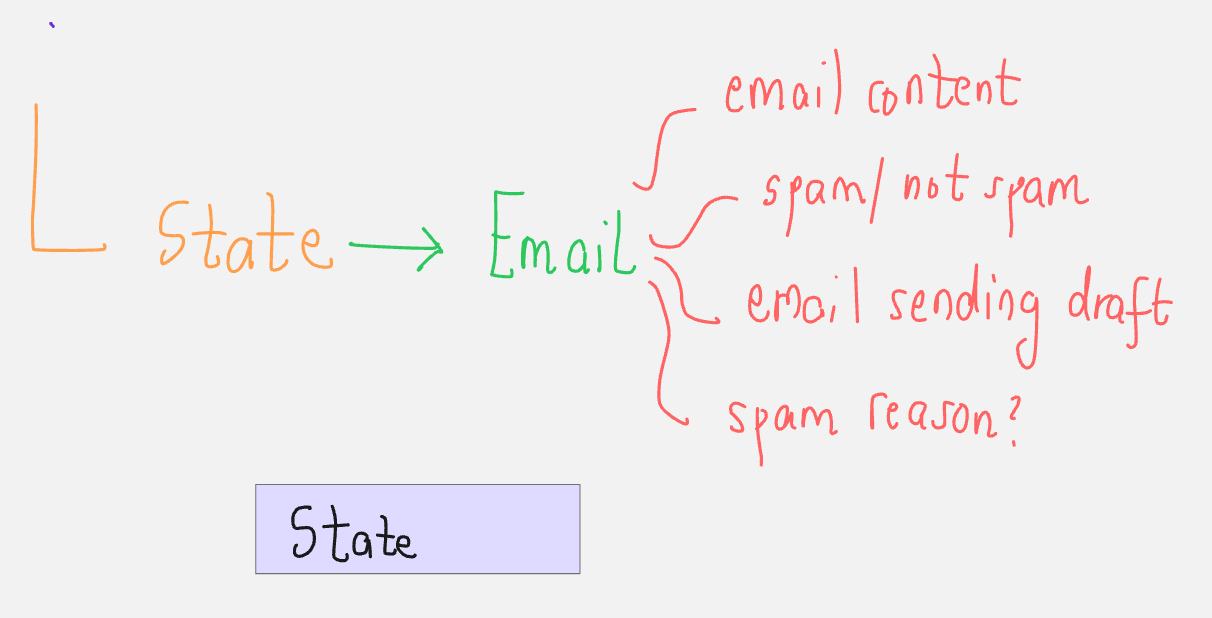
\includegraphics[width=0.8\linewidth,keepaspectratio]{aiagents72}
	
        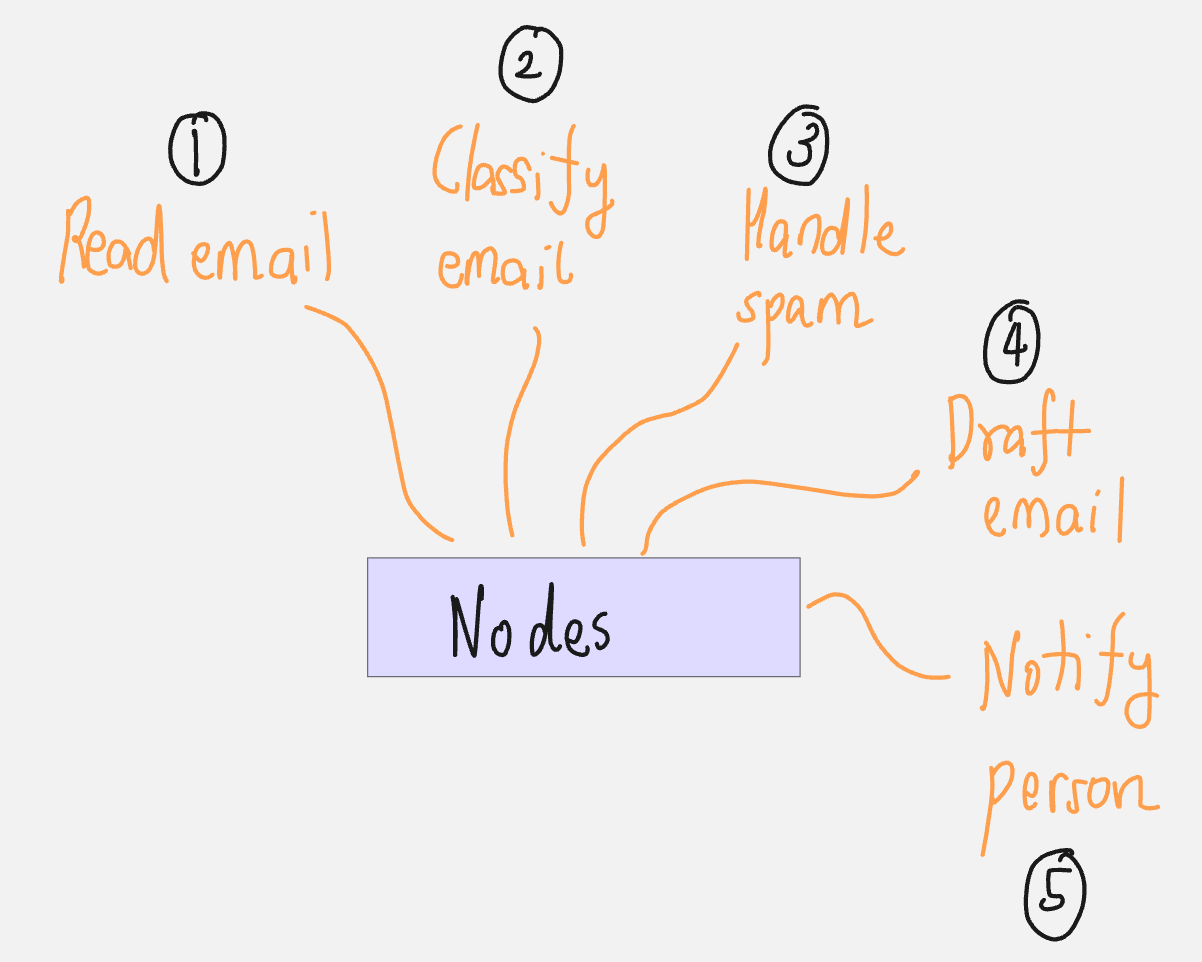
\includegraphics[width=0.8\linewidth,keepaspectratio]{aiagents73}
		
		{\tiny (Ref: Vizuara AI Agents Bootcamp)}
				
        \end{center}    
    \end{column}
    \begin{column}[T]{0.5\linewidth}
        \begin{center}

        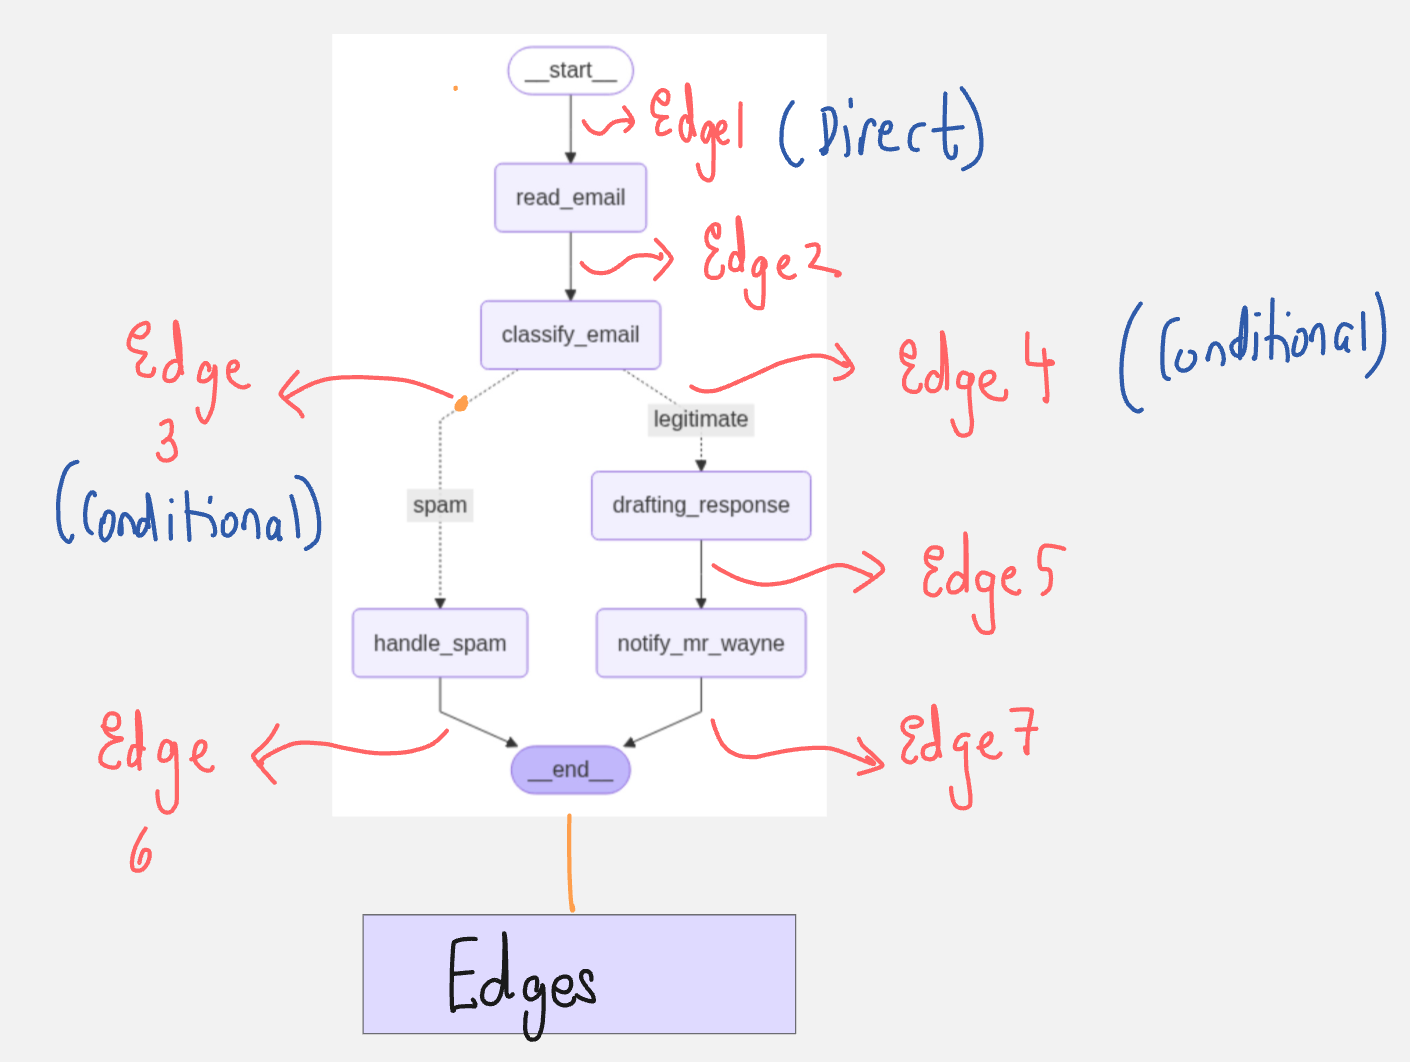
\includegraphics[width=0.8\linewidth,keepaspectratio]{aiagents74}
		
		{\tiny (Ref: Vizuara AI Agents Bootcamp)}
				
        \end{center}    
    \end{column}
  \end{columns}
\end{frame}

%%%%%%%%%%%%%%%%%%%%%%%%%%%%%%%%%%%%%%%%%%%%%%%%%%%%%%%%%%%
\begin{frame}[fragile]\frametitle{LangGraph}

        \begin{center}

        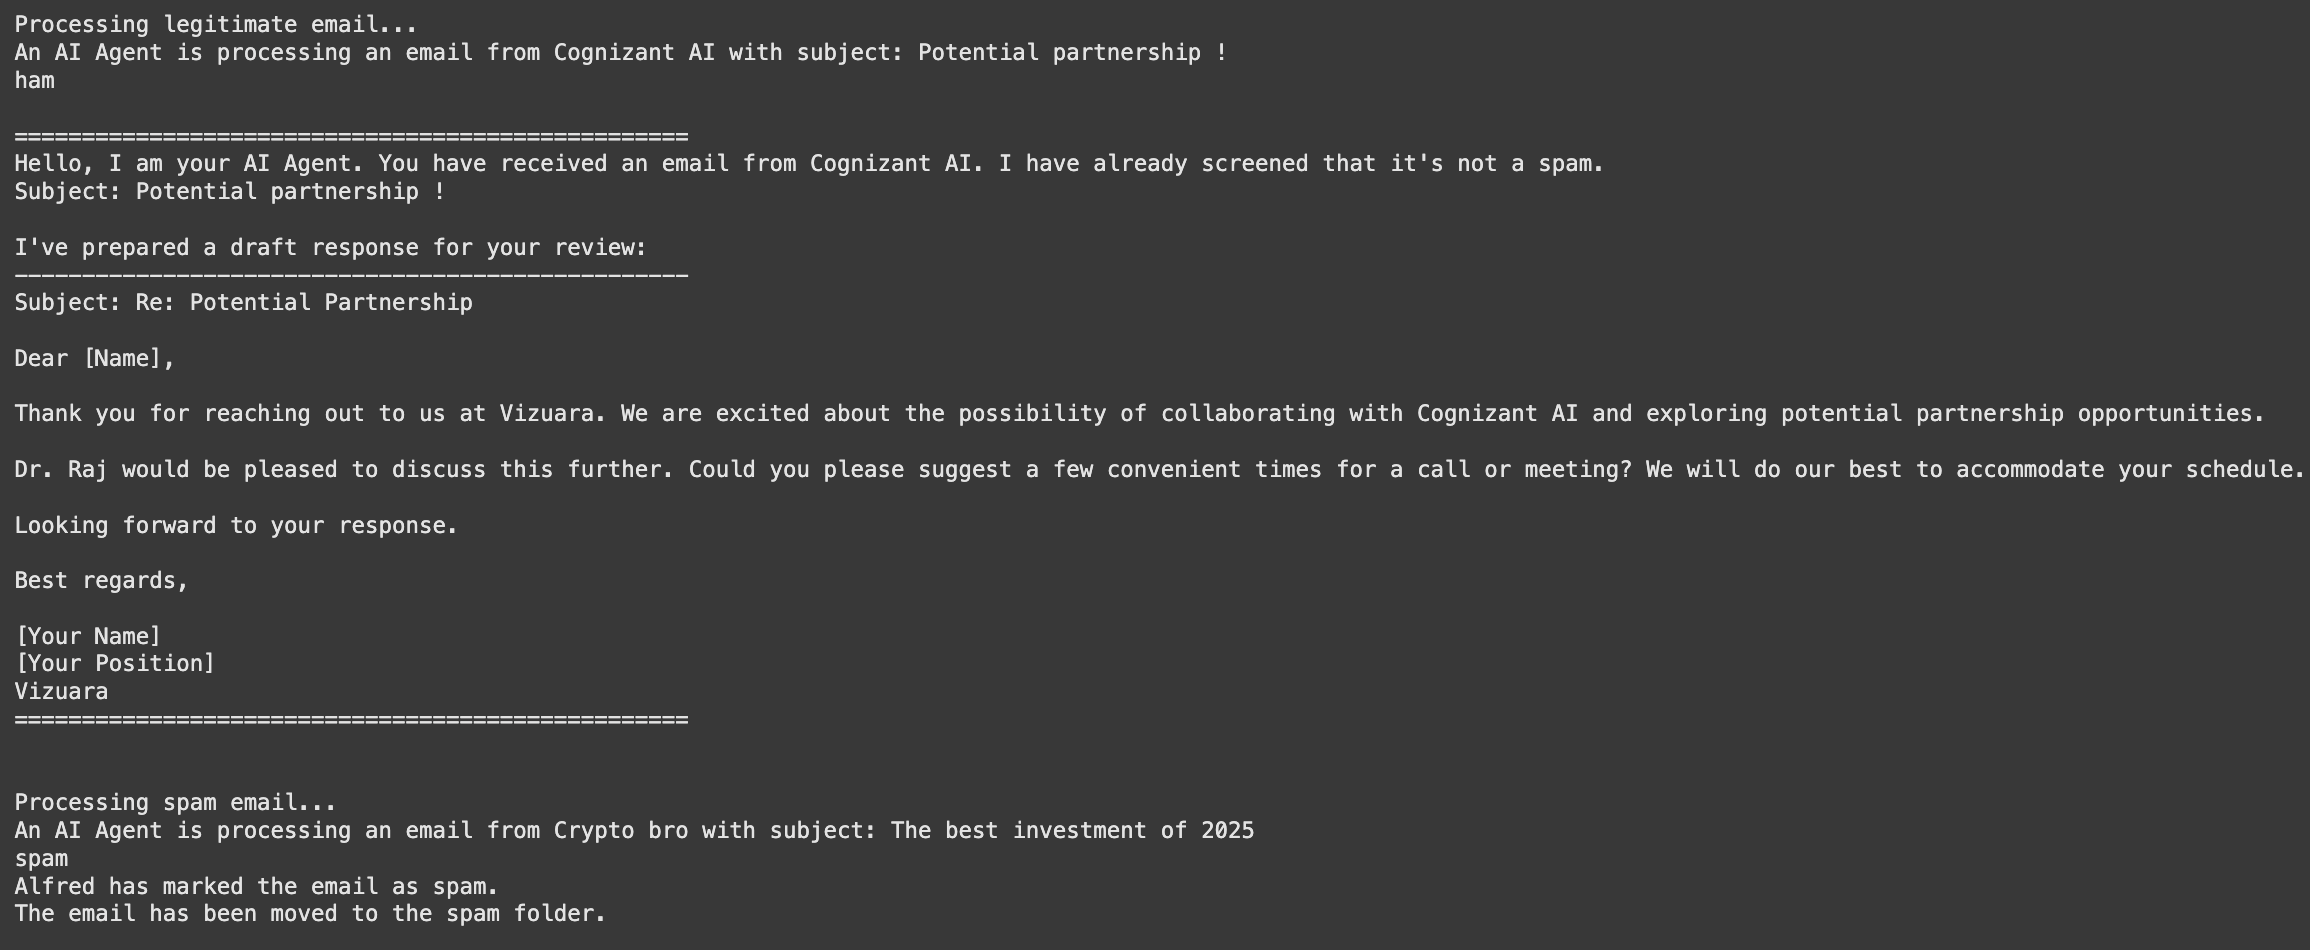
\includegraphics[width=\linewidth,keepaspectratio]{aiagents75}
		
		{\tiny (Ref: Vizuara AI Agents Bootcamp)}
				
        \end{center}    

\end{frame}


%%%%%%%%%%%%%%%%%%%%%%%%%%%%%%%%%%%%%%%%%%%%%%%%%%%%%%%%%%%%%%%%%%%%%%%%%%%%%%%%%%
\begin{frame}\frametitle{Concepts}

\begin{itemize}
\item Model: Large Language Model that supports Function Calling
\item Tools: Actions taken by app, ie API calls, Db operations, etc
\item State: Represents info that is carried though out the workflow e.g Message State has list of messages produced from each Node.
\item Node: executable logic container, a Langchain runnable or a Tool invoker. Nodes are connected by edges.
\item Edge: control flow of info, conditional or normal
\item Workflow: The graph, having nodes and edges, can be invoked or streamed from.
\end{itemize}

\begin{center}
\includegraphics[width=0.8\linewidth,keepaspectratio]{langgraph2}
\end{center}	  

{\tiny (Ref: Introduction to LangGraph | Building an AI Generated Podcast - Prompt Circle AI)}
\end{frame}

%%%%%%%%%%%%%%%%%%%%%%%%%%%%%%%%%%%%%%%%%%%%%%%%%%%%%%%%%%%
\begin{frame}[fragile]\frametitle{Graph and State Machine Concepts}
      \begin{itemize}
        \item State: System's behavioral condition (hunger, sleep, temperature)
        \item Events: Actions that trigger state changes (feeding, soothing)
        \item Nodes: Decision-makers and executors in the workflow
        \item Baby care analogy: Mother decides, elders check, father executes
        \item State updates trigger continuous decision-making cycles
        \item Graph structure provides flexible workflow representation
        \item State machines enable dynamic routing based on conditions
        \item More intuitive than linear processing chains
      \end{itemize}
\end{frame}

%%%%%%%%%%%%%%%%%%%%%%%%%%%%%%%%%%%%%%%%%%%%%%%%%%%%%%%%%%%
\begin{frame}[fragile]\frametitle{LangGraph Core Features}
      \begin{itemize}
        \item Looping and branching capabilities with conditional statements
        \item State persistence with automatic save and restore functionality
        \item Human-machine interaction support with review and editing
        \item Streaming processing for real-time feedback and status updates
        \item Seamless integration with existing LangChain components
        \item Support for LCEL expressions and rich tool ecosystem
        \item Flexible interaction control mechanisms
        \item Enhanced user experience through responsive design
      \end{itemize}
\end{frame}

%%%%%%%%%%%%%%%%%%%%%%%%%%%%%%%%%%%%%%%%%%%%%%%%%%%%%%%%%%%
\begin{frame}[fragile]\frametitle{Core Concept: State}

      \begin{itemize}
        \item State is the foundation of LangGraph applications
        \item Can be simple dictionary or Pydantic model
        \item Contains all information needed during runtime
        \item Passed between nodes and updated throughout execution
      \end{itemize}
	  
      \begin{lstlisting}[language=Python, basicstyle=\small]
from typing import List, Dict
from pydantic import BaseModel

class ChatState(BaseModel):
    messages: List[Dict[str, str]] = []
    current_input: str = ""
    tools_output: Dict[str, str] = {}
    final_response: str = ""
      \end{lstlisting}

\end{frame}

%%%%%%%%%%%%%%%%%%%%%%%%%%%%%%%%%%%%%%%%%%%%%%%%%%%%%%%%%%%
\begin{frame}[fragile]\frametitle{Core Concept: Nodes}
Nodes are Python functions used to process state and return updated state:



      \begin{lstlisting}[language=Python, basicstyle=\small]
async def process_input(state: ChatState) -> ChatState:
    # Process user input
    messages = state.messages + [{"role": "user", "content": state.current_input}]
    return ChatState(
        messages=messages,
        current_input=state.current_input,
        tools_output=state.tools_output)

async def generate_response(state: ChatState) -> ChatState:
    # Generate response using LLM
    response = await llm.ainvoke(state.messages)
    messages = state.messages + [{"role": "assistant", "content": response}]
    return ChatState(
        messages=messages,
        current_input=state.current_input,
        tools_output=state.tools_output,
        final_response=response)
      \end{lstlisting}
\end{frame}

%%%%%%%%%%%%%%%%%%%%%%%%%%%%%%%%%%%%%%%%%%%%%%%%%%%%%%%%%%%
\begin{frame}[fragile]\frametitle{Core Concept: Edges}

      \begin{itemize}
        \item Edges define connections and routing logic between nodes
        \item Support conditional routing based on state
        \item Enable dynamic execution paths
      \end{itemize}
	  
      \begin{lstlisting}[language=Python, basicstyle=\small]
from langgraph.graph import StateGraph, END

# Create graph structure
workflow = StateGraph(ChatState)

# Add nodes
workflow.add_node("process_input", process_input)
workflow.add_node("generate_response", generate_response)

# Define edges and routing logic
workflow.add_edge("process_input", "generate_response")
workflow.add_edge("generate_response", END)
      \end{lstlisting}

\end{frame}


%%%%%%%%%%%%%%%%%%%%%%%%%%%%%%%%%%%%%%%%%%%%%%%%%%%%%%%%%%%
\begin{frame}[fragile]\frametitle{Building the Chatbot Graph}

This example demonstrates the basic usage of LangGraph:
      \begin{itemize}
        \item Define state model
        \item Create processing nodes
        \item Build the graph structure
        \item Define routing logic
        \item Compile and run
      \end{itemize}
\end{frame}

%%%%%%%%%%%%%%%%%%%%%%%%%%%%%%%%%%%%%%%%%%%%%%%%%%%%%%%%%%%
\begin{frame}[fragile]\frametitle{Simple Chatbot Implementation}
      \begin{lstlisting}[language=Python, basicstyle=\tiny]
from typing import List, Dict
from pydantic import BaseModel
from langgraph.graph import StateGraph, END
from langchain_core.language_models import ChatOpenAI

class ChatState(BaseModel):
    messages: List[Dict[str, str]] = []
    current_input: str = ""
    should_continue: bool = True

async def process_user_input(state: ChatState) -> ChatState:
    messages = state.messages + [{"role": "user", "content": state.current_input}]
    return ChatState(
        messages=messages,
        current_input=state.current_input,
        should_continue=True
    )

async def generate_ai_response(state: ChatState) -> ChatState:
    llm = ChatOpenAI(temperature=0.7)
    response = await llm.ainvoke(state.messages)
    messages = state.messages + [{"role": "assistant", "content": response}]
    return ChatState(
        messages=messages,
        current_input=state.current_input,
        should_continue=True
    )

def should_continue(state: ChatState) -> str:
    if "goodbye" in state.current_input.lower():
        return "end"
    return "continue"
      \end{lstlisting}
\end{frame}

%%%%%%%%%%%%%%%%%%%%%%%%%%%%%%%%%%%%%%%%%%%%%%%%%%%%%%%%%%%
\begin{frame}[fragile]\frametitle{Building the Chatbot Graph}
      \begin{lstlisting}[language=Python, basicstyle=\tiny]
# Build the graph
workflow = StateGraph(ChatState)

# Add nodes
workflow.add_node("process_input", process_user_input)
workflow.add_node("generate_response", generate_ai_response)

# Add edges
workflow.add_edge("process_input", "generate_response")
workflow.add_conditional_edges("generate_response", should_continue, 
    {"continue": "process_input", "end": END})

# Compile the graph
app = workflow.compile()

# Run the conversation
async def chat():
    state = ChatState()
    while True:
        user_input = input("You: ")
        state.current_input = user_input
        state = await app.ainvoke(state)
        print("Bot:", state.messages[-1]["content"])
        if not state.should_continue:
            break

# Run chat
import asyncio
asyncio.run(chat())			
      \end{lstlisting}
\end{frame}



%%%%%%%%%%%%%%%%%%%%%%%%%%%%%%%%%%%%%%%%%%%%%%%%%%%%%%%%%%%%%%%%%%%%%%%%%%%%%%%%%%
\begin{frame}[fragile]\frametitle{}
\begin{center}
{\Large Applications}
\end{center}
\end{frame}


%%%%%%%%%%%%%%%%%%%%%%%%%%%%%%%%%%%%%%%%%%%%%%%%%%%%%%%%%%%%%%%%%%%%%%%%%%%%%%%%%%
\begin{frame}\frametitle{Podcast Generator}

\begin{center}
\includegraphics[width=0.8\linewidth,keepaspectratio]{langgraph3}
\end{center}	  


{\tiny (Ref: Introduction to LangGraph | Building an AI Generated Podcast - Prompt Circle AI)}

Code at https://github.com/hollaugo/langgraph-framework-tutorial
\end{frame}


%%%%%%%%%%%%%%%%%%%%%%%%%%%%%%%%%%%%%%%%%%%%%%%%%%%%%%%%%%%%%%%%%%%%%%%%%%%%%%%%%%
\begin{frame}[fragile]\frametitle{News Aggregator}

\begin{center}
\includegraphics[width=0.8\linewidth,keepaspectratio]{langgraph4}
\end{center}	

Code: https://github.com/rajib76/multi\_agent/blob/main/01\_how\_to\_langgraph\_example\_01.py

{\tiny (Ref: Langgraph: The Agent Orchestrator - Rajib Deb)}


\end{frame}

%%%%%%%%%%%%%%%%%%%%%%%%%%%%%%%%%%%%%%%%%%%%%%%%%%%%%%%%%%%%%%%%%%%%%%%%%%%%%%%%%%
\begin{frame}[fragile]\frametitle{}
\begin{center}
{\Large Agents using LangGraph}
\end{center}
\end{frame}

%%%%%%%%%%%%%%%%%%%%%%%%%%%%%%%%%%%%%%%%%%%%%%%%%%%%%%%%%%%
\begin{frame}[fragile]\frametitle{Creating a Vision Assistant Agent}
\begin{columns}
    \begin{column}[T]{0.7\linewidth}
      \begin{itemize}
        \item Vision-enabled agent implementing explicit "Thought → Action → Observation" loop
        \item \textbf{AgentState:} Stores input\_file (image path) and messages list for conversation history
        \item \textbf{Assistant node:} GPT-4 with vision capability bound to image analysis and math tools
        \item \textbf{Tools node:} Executes tool functions (extract\_text, divide) and records results
        \item Assistant decides to use tools or provide final answer based on task requirements
        \item Conditional edge uses tools\_condition to route between assistant and tools nodes
        \item Creates cycle: assistant thinks → tool execution → assistant processes results → repeat
        \item Loop continues until assistant provides final answer without requesting tools
      \end{itemize}
    \end{column}
    \begin{column}[T]{0.3\linewidth}
        \begin{center}
        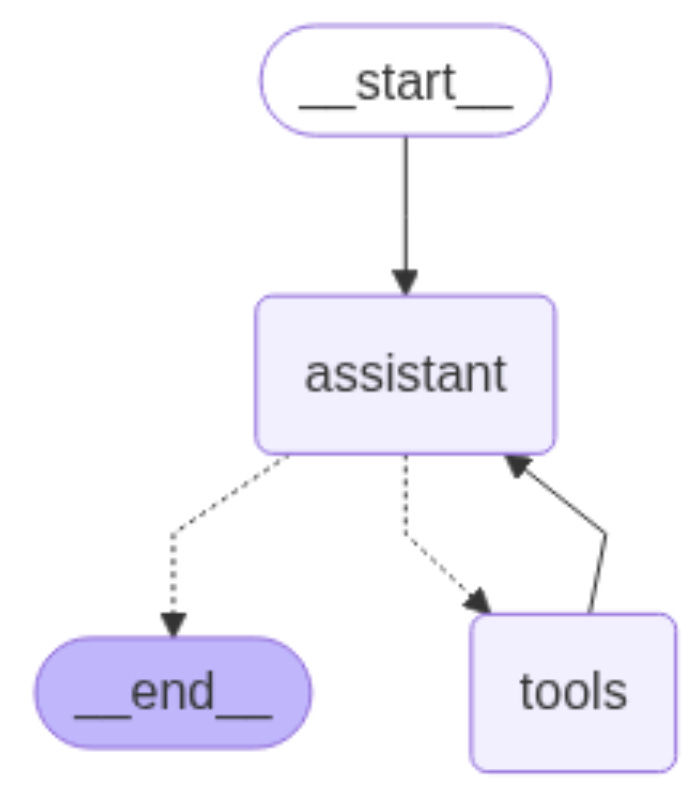
\includegraphics[width=\linewidth,keepaspectratio]{aiagents76}
        \end{center}    
    \end{column}
  \end{columns}
\end{frame}

%%%%%%%%%%%%%%%%%%%%%%%%%%%%%%%%%%%%%%%%%%%%%%%%%%%%%%%%%%%
\begin{frame}[fragile]\frametitle{Creating a Vision Assistant Agent}

        \begin{center}

        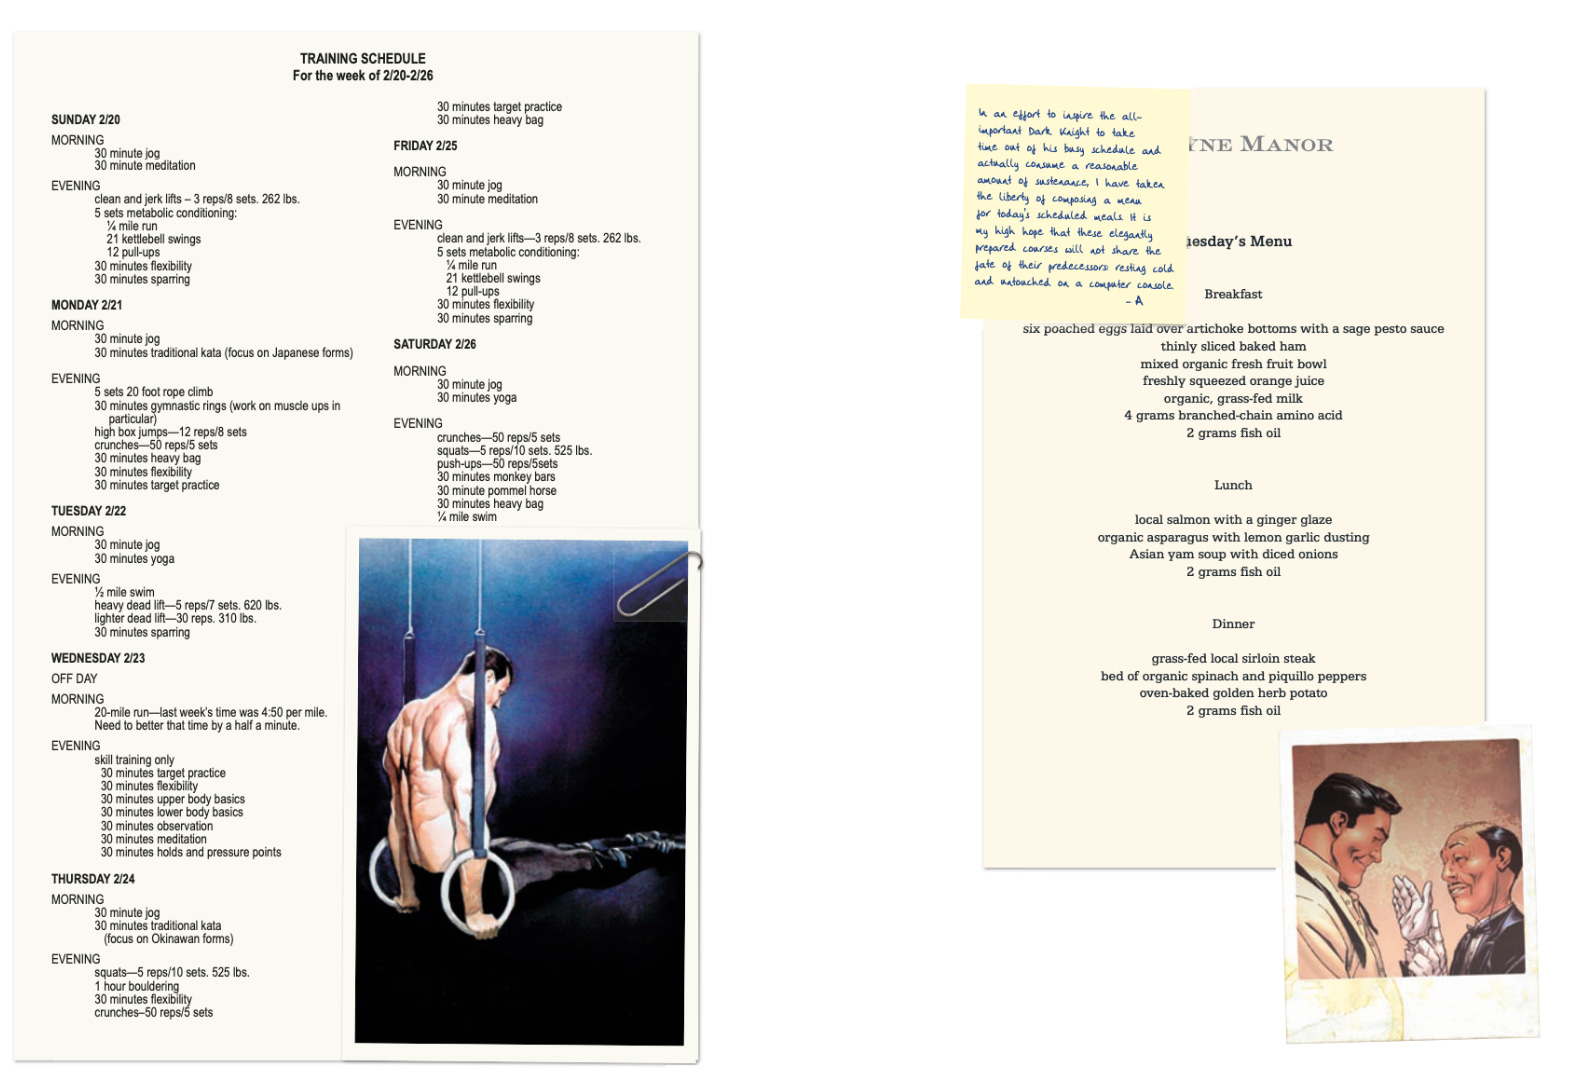
\includegraphics[width=0.9\linewidth,keepaspectratio]{aiagents77}
		
		{\tiny (Ref: Vizuara AI Agents Bootcamp)}
				
        \end{center}    

\end{frame}

%%%%%%%%%%%%%%%%%%%%%%%%%%%%%%%%%%%%%%%%%%%%%%%%%%%%%%%%%%%
\begin{frame}[fragile]\frametitle{Creating a Vision Assistant Agent}

        \begin{center}

        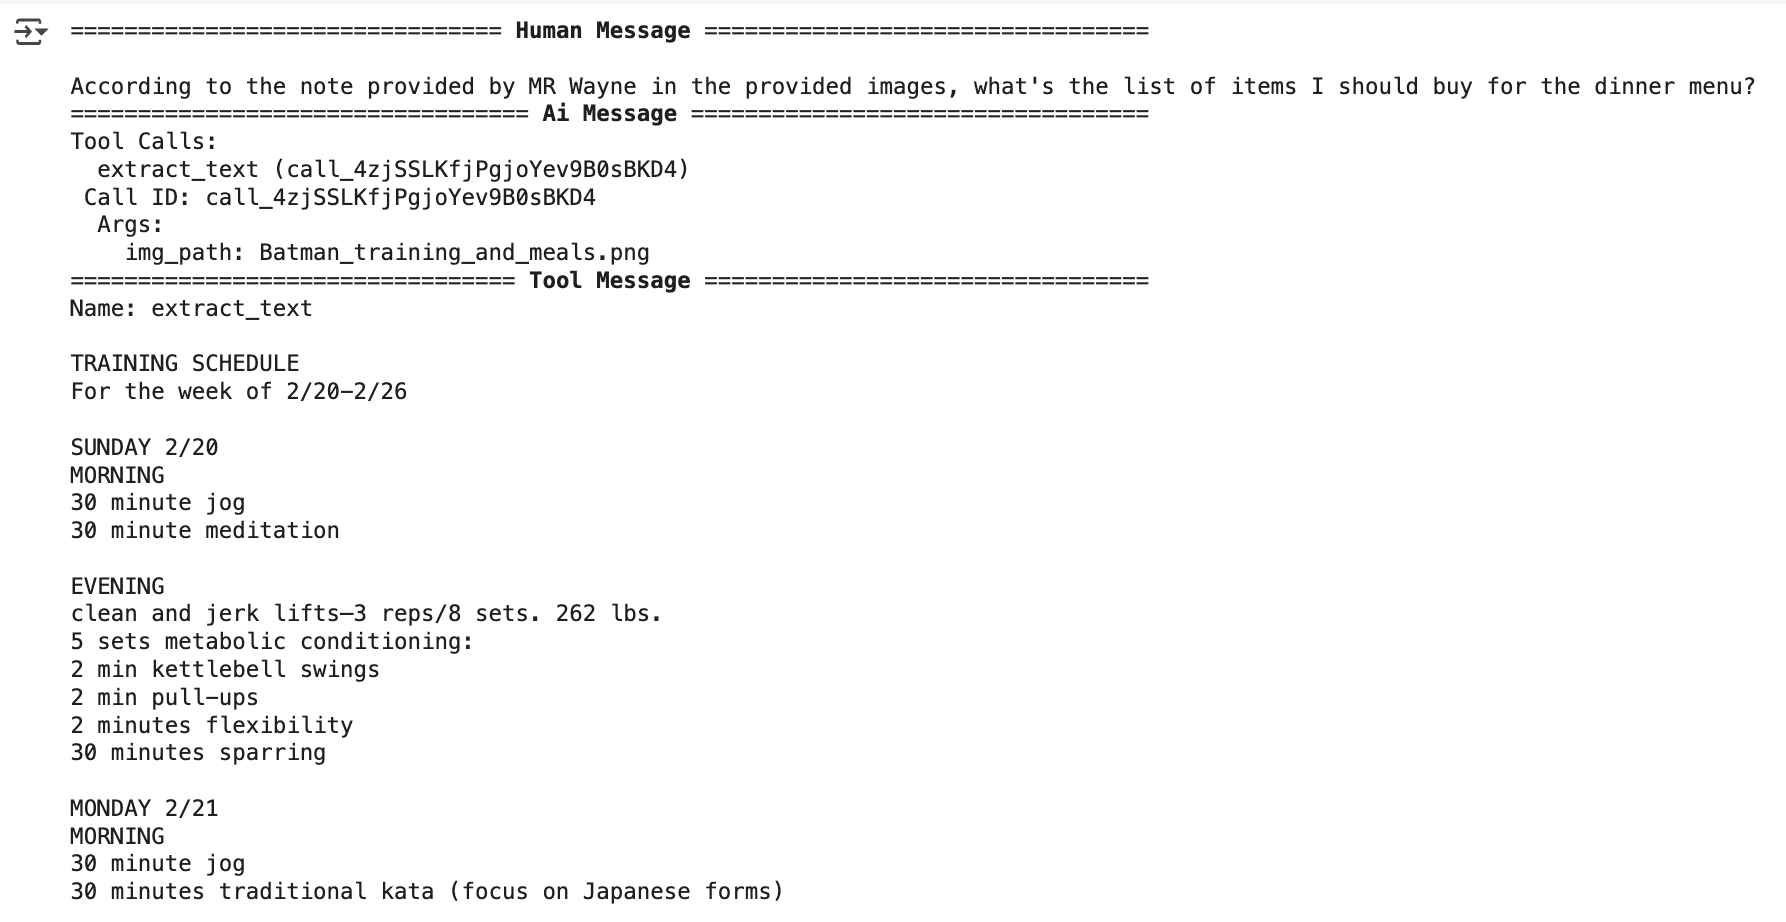
\includegraphics[width=\linewidth,keepaspectratio]{aiagents78}
		
		{\tiny (Ref: Vizuara AI Agents Bootcamp)}
				
        \end{center}    

\end{frame}



%%%%%%%%%%%%%%%%%%%%%%%%%%%%%%%%%%%%%%%%%%%%%%%%%%%%%%%%%%%
\begin{frame}[fragile]\frametitle{Tracing Agent Workflows with Langfuse}

      \begin{itemize}
        \item Observability crucial for debugging complex agent behaviors with multiple steps
        \item \textbf{Traces:} Detailed execution records capturing prompts, responses, paths, and tool usage
        \item Langfuse provides user-friendly dashboard for inspecting agent workflow traces
        \item Integrates via OpenTelemetry standards with tracing callbacks in LangGraph code
        \item Enables monitoring of both email agent and vision agent execution flows
        \item Tools-assistant loop clearly visible in Langfuse trace visualization
        \item Answers "why did my agent do X?" through accessible trace inspection
        \item Essential best practice for moving from prototypes to production-grade AI systems
      \end{itemize}

\end{frame}

%%%%%%%%%%%%%%%%%%%%%%%%%%%%%%%%%%%%%%%%%%%%%%%%%%%%%%%%%%%
\begin{frame}[fragile]\frametitle{Tracing Agent Workflows with Langfuse}

        \begin{center}

        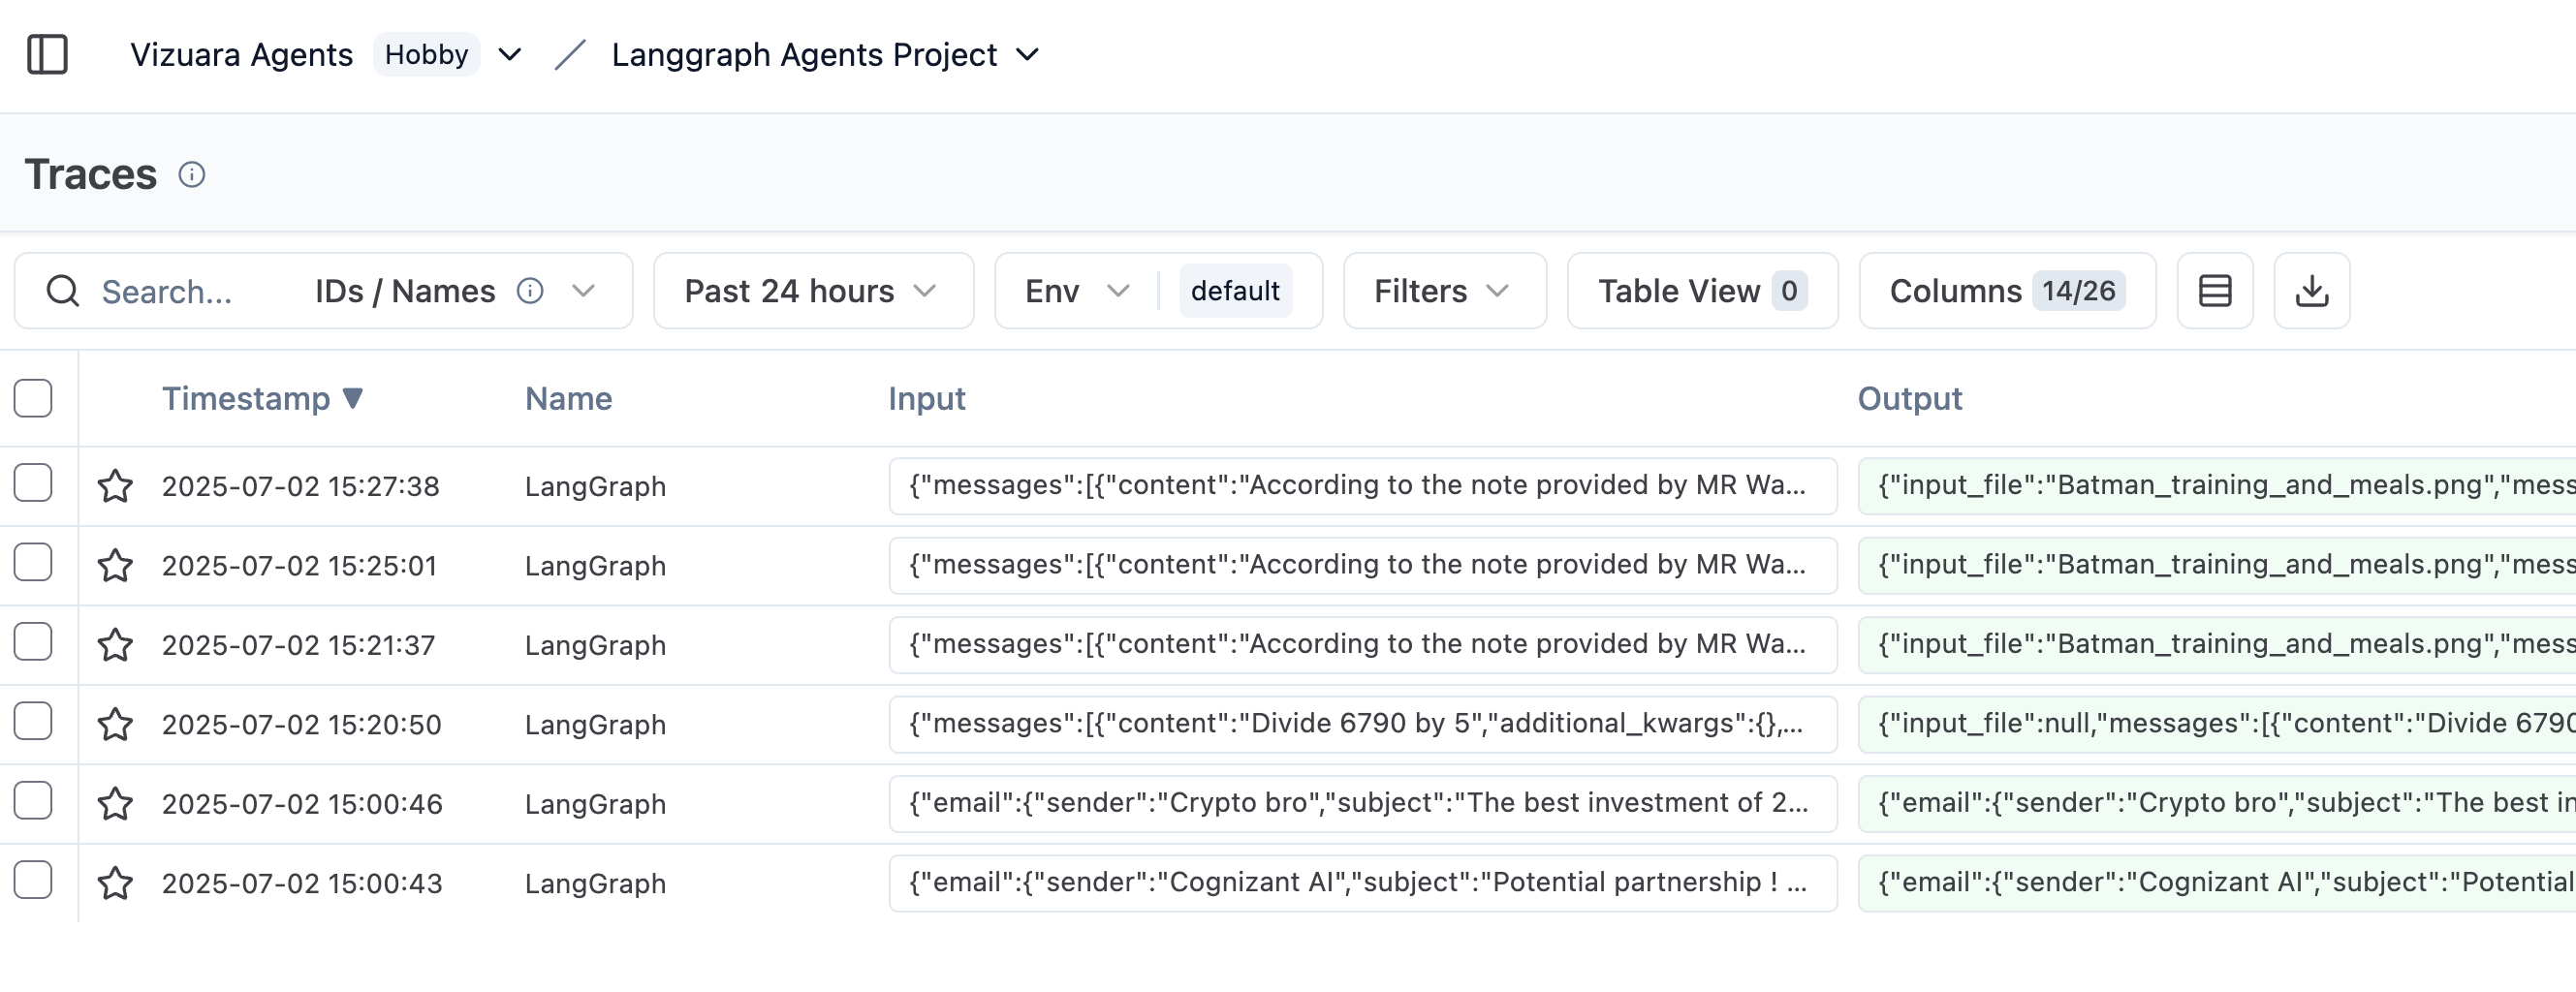
\includegraphics[width=\linewidth,keepaspectratio]{aiagents79}
		
		{\tiny (Ref: Vizuara AI Agents Bootcamp)}
				
        \end{center}    

\end{frame}

%%%%%%%%%%%%%%%%%%%%%%%%%%%%%%%%%%%%%%%%%%%%%%%%%%%%%%%%%%%
\begin{frame}[fragile]\frametitle{Tracing Agent Workflows with Langfuse}

        \begin{center}

        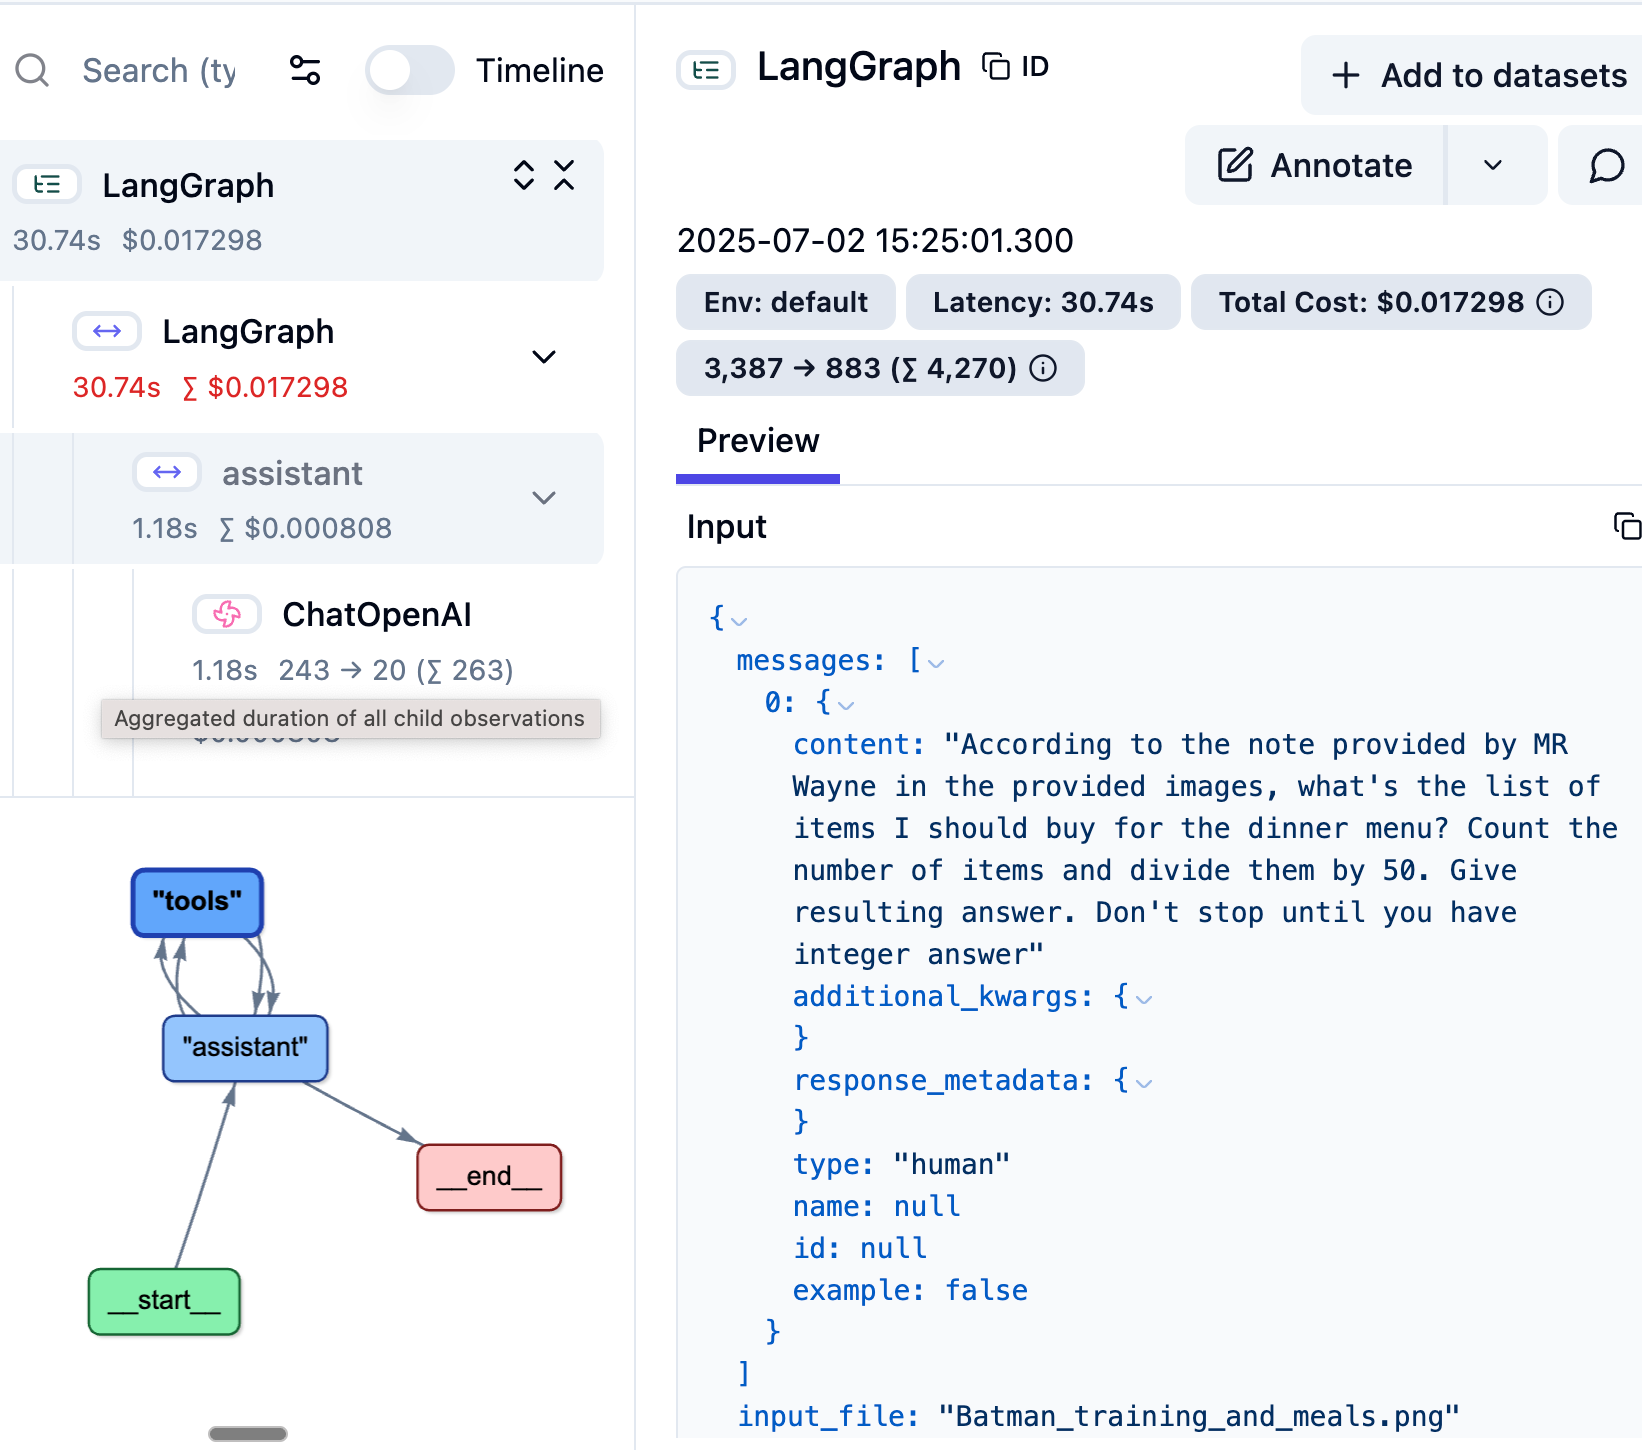
\includegraphics[width=0.7\linewidth,keepaspectratio]{aiagents80}
		
		{\tiny (Ref: Vizuara AI Agents Bootcamp)}
				
        \end{center}    

\end{frame}


%%%%%%%%%%%%%%%%%%%%%%%%%%%%%%%%%%%%%%%%%%%%%%%%%%%%%%%%%%%
\begin{frame}[fragile]\frametitle{Best Practices}

      \begin{itemize}
        \item State Design: Keep the state model simple and clear, only including necessary information. Use type hints to increase code readability.
        \item Node Functions: Maintain single responsibility, handle exceptions, and return new state objects instead of modifying existing state.
        \item Edge Design: Use clear conditional logic, avoid complex cyclic dependencies, and consider all possible paths.
        \item Error Handling: Add error handling at critical nodes, provide fallback mechanisms, and log detailed error information.
      \end{itemize}
\end{frame}
